%\section{Einleitung}

{
	\usebackgroundtemplate{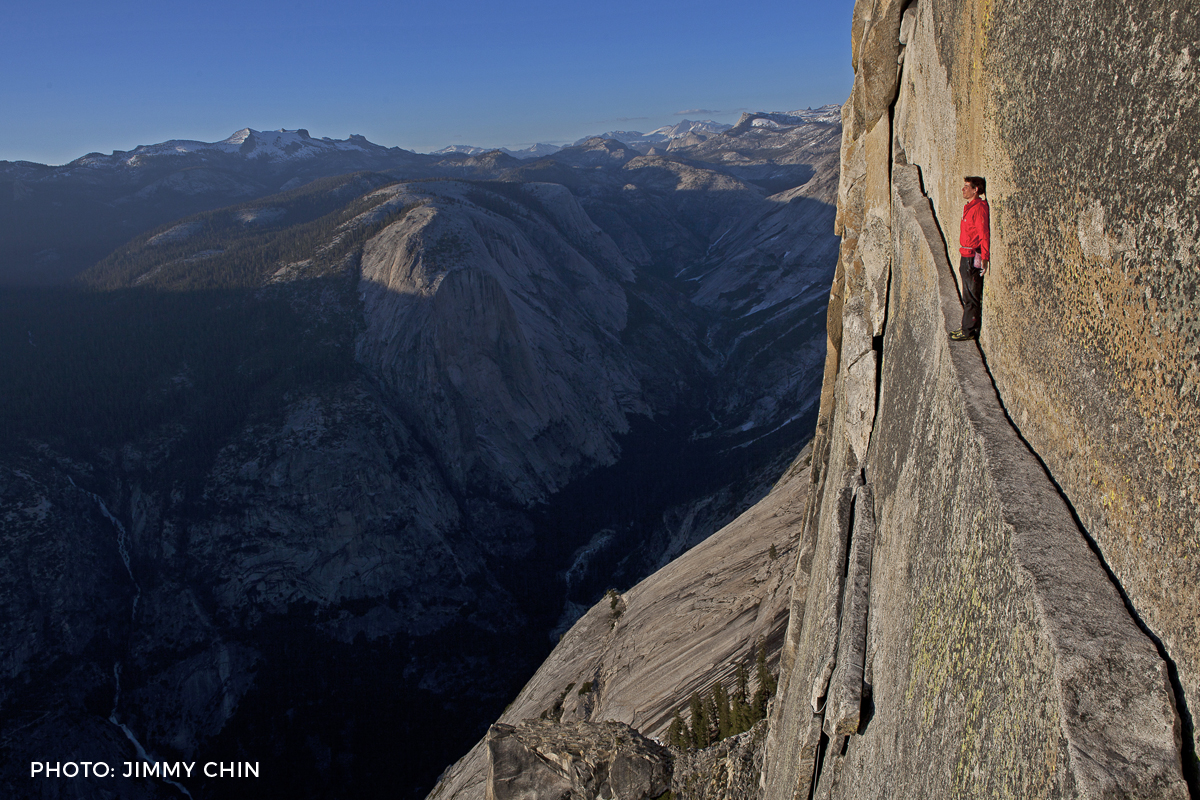
\includegraphics[width=\paperwidth]{include/images/honnold.jpg}}
	\begin{frame}[standout]
		\begin{textblock}{50}(-10,83)
			\href{http://www.accidentofgeography.com/alex-honnold-epic-el-capitan-triumph/}{	\textcolor{tertiary}{{\small \textcopyright Jimmy Chin}}} 
		\end{textblock}
	\end{frame}
}

\begin{frame}[standout]
\begin{figure}[h]
	\centering
	\begin{subfigure}[t]{0.49\columnwidth}
		\centering
		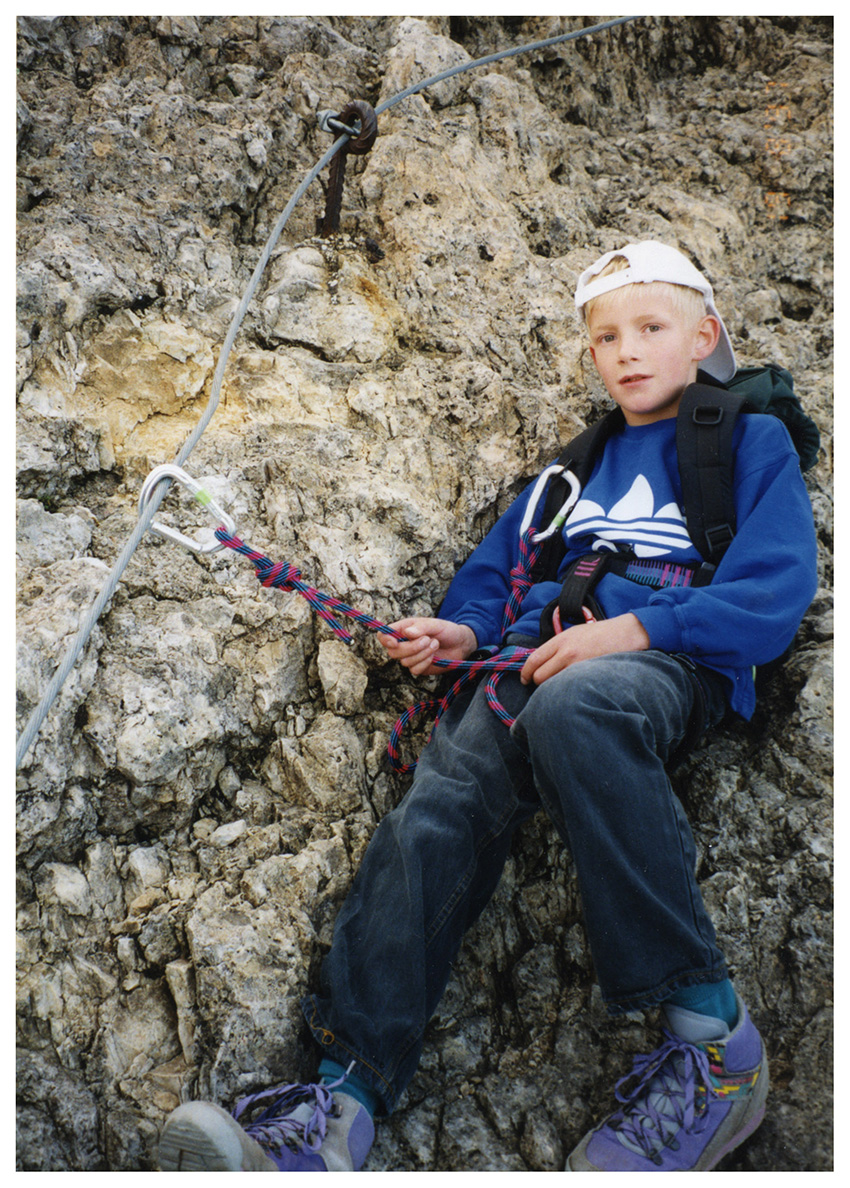
\includegraphics[angle=7,width=\textwidth]{include/images/1997.jpg}
	\end{subfigure}
	\hspace*{\fill}
	\begin{subfigure}[t]{0.49\columnwidth}
		\centering
		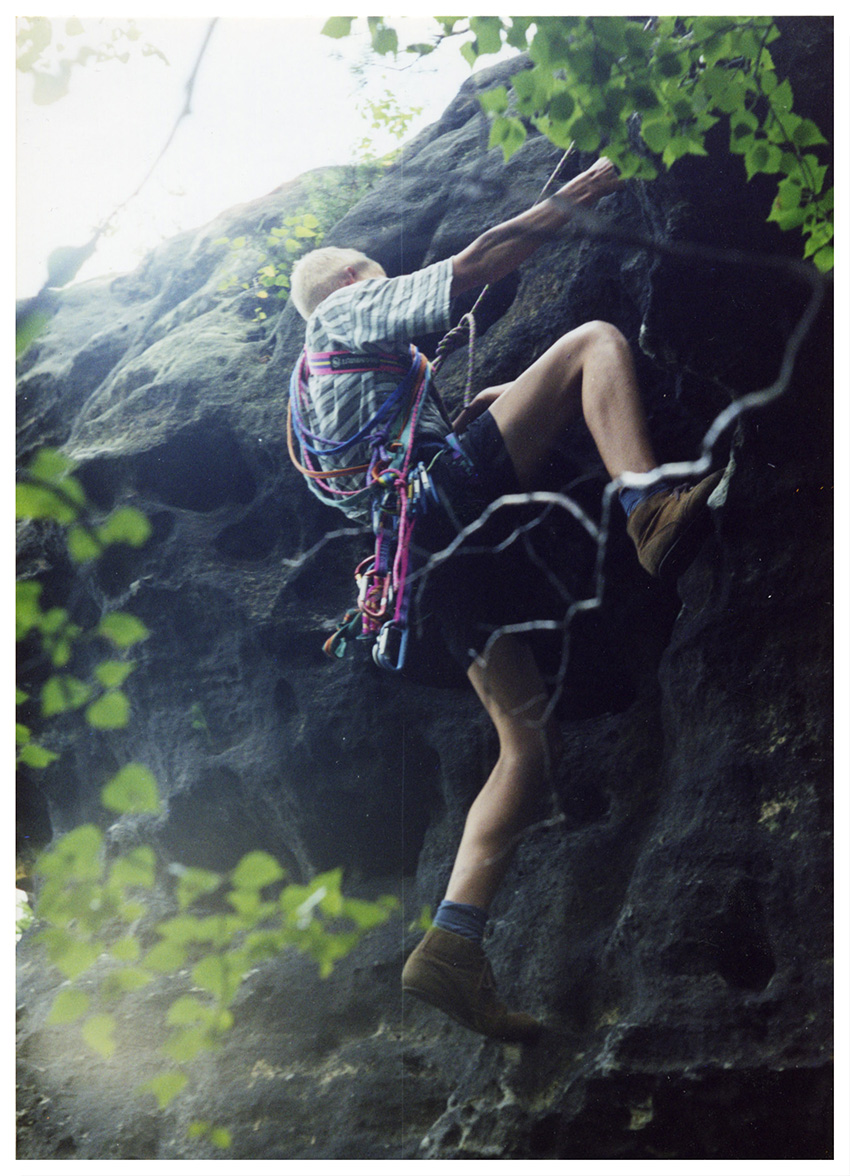
\includegraphics[angle=-5,width=\textwidth]{include/images/2002.jpg}
	\end{subfigure}
\end{figure}
\end{frame}

{
	\usebackgroundtemplate{\movie[label=clip-1,width=\paperwidth,height=\paperheight,open,once,showcontrols=false]{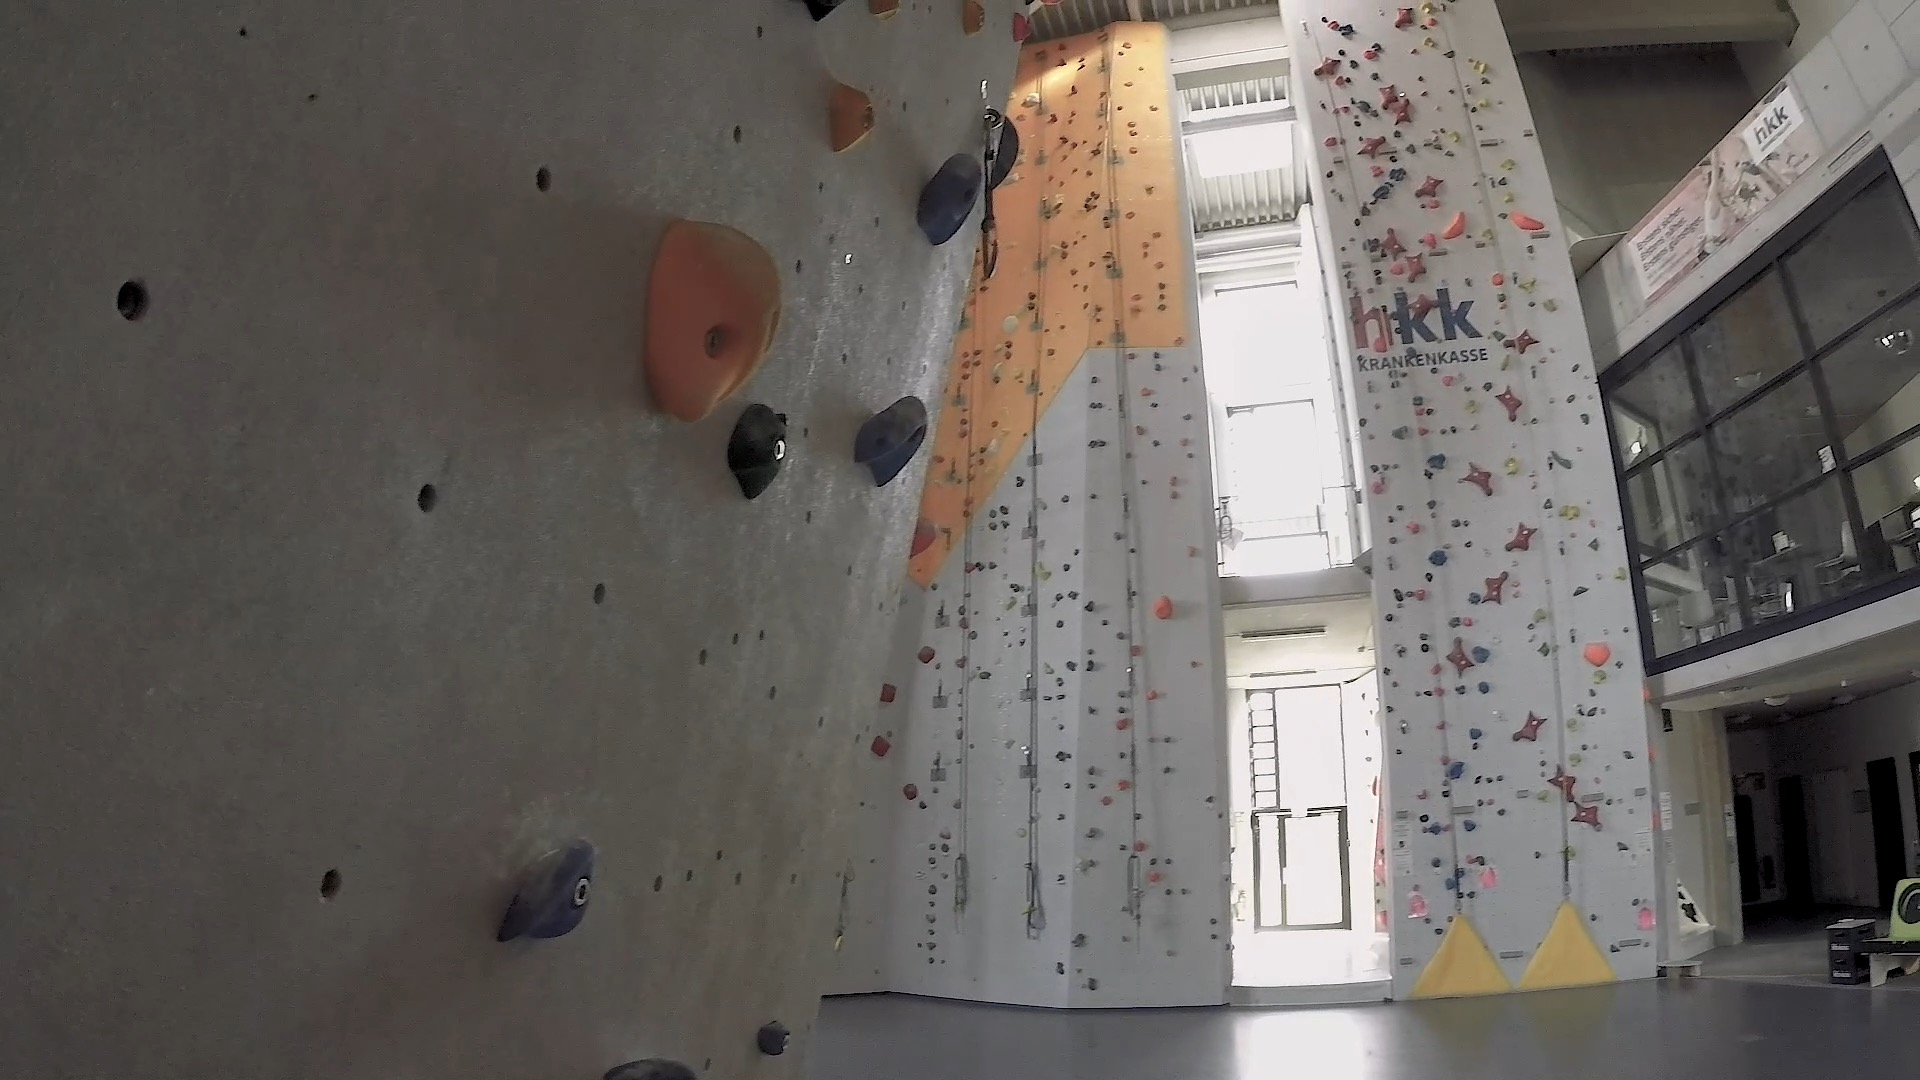
\includegraphics[width=\paperwidth]{include/images/master-thesis-clip-1.jpg}}{include/videos/master-thesis-clip-1.mov}}
	\begin{frame}[standout]
	\end{frame}
}

\begin{frame}{Lässt sich \textcolor{tertiary}{Sturzangst}, wie auch Höhenangst, \textcolor{tertiary}{in VR} auslösen?}
	\centering
	\begin{overpic}[height=0.8\textheight]{include/images/samsung-gear-acrophobia-original.jpg}
		\rbox{-4}{1}{\textcolor{source}{\tiny{Quelle: \href{https://vrscout.com/projects/fear-of-heights-samsung-gear-vr/}{VRscout}}}}
	\end{overpic}
\end{frame}

\begin{frame}{Related Work mit \textcolor{tertiary}{Höhen} und \textcolor{tertiary}{Kanten}}
\begin{columns}
	\begin{column}{0.45\textwidth}
		\begin{center}
			\begin{overpic}[height=0.8\textheight]{include/images/pijpers.jpg}
				\rbox{-15}{1}{\textcolor{black}{\tiny{Quelle: \href{https://www.researchgate.net/figure/Side-view-of-the-virtual-environment-Subjects-start-in-the-Training-Room-and-later-enter_fig1_247181822}{ResearchGate}}}}
			\end{overpic}
		\end{center}
	\end{column}
	\begin{column}{0.55\textwidth}
		\begin{center}
			\begin{overpic}[height=0.8\textheight]{include/images/meehan.jpg}
				\rbox{-1}{1}{\textcolor{source}{\tiny{Quelle: \href{https://www.researchgate.net/figure/View-of-the-20-in-pit-from-the-wooden-ledge_fig3_7596875}{ResearchGate}}}}
			\end{overpic}
		\end{center}
	\end{column}
\end{columns}
\end{frame}

{
	\usebackgroundtemplate{\movie[label=clip-1,width=\paperwidth,height=\paperheight,open,once,showcontrols=false]{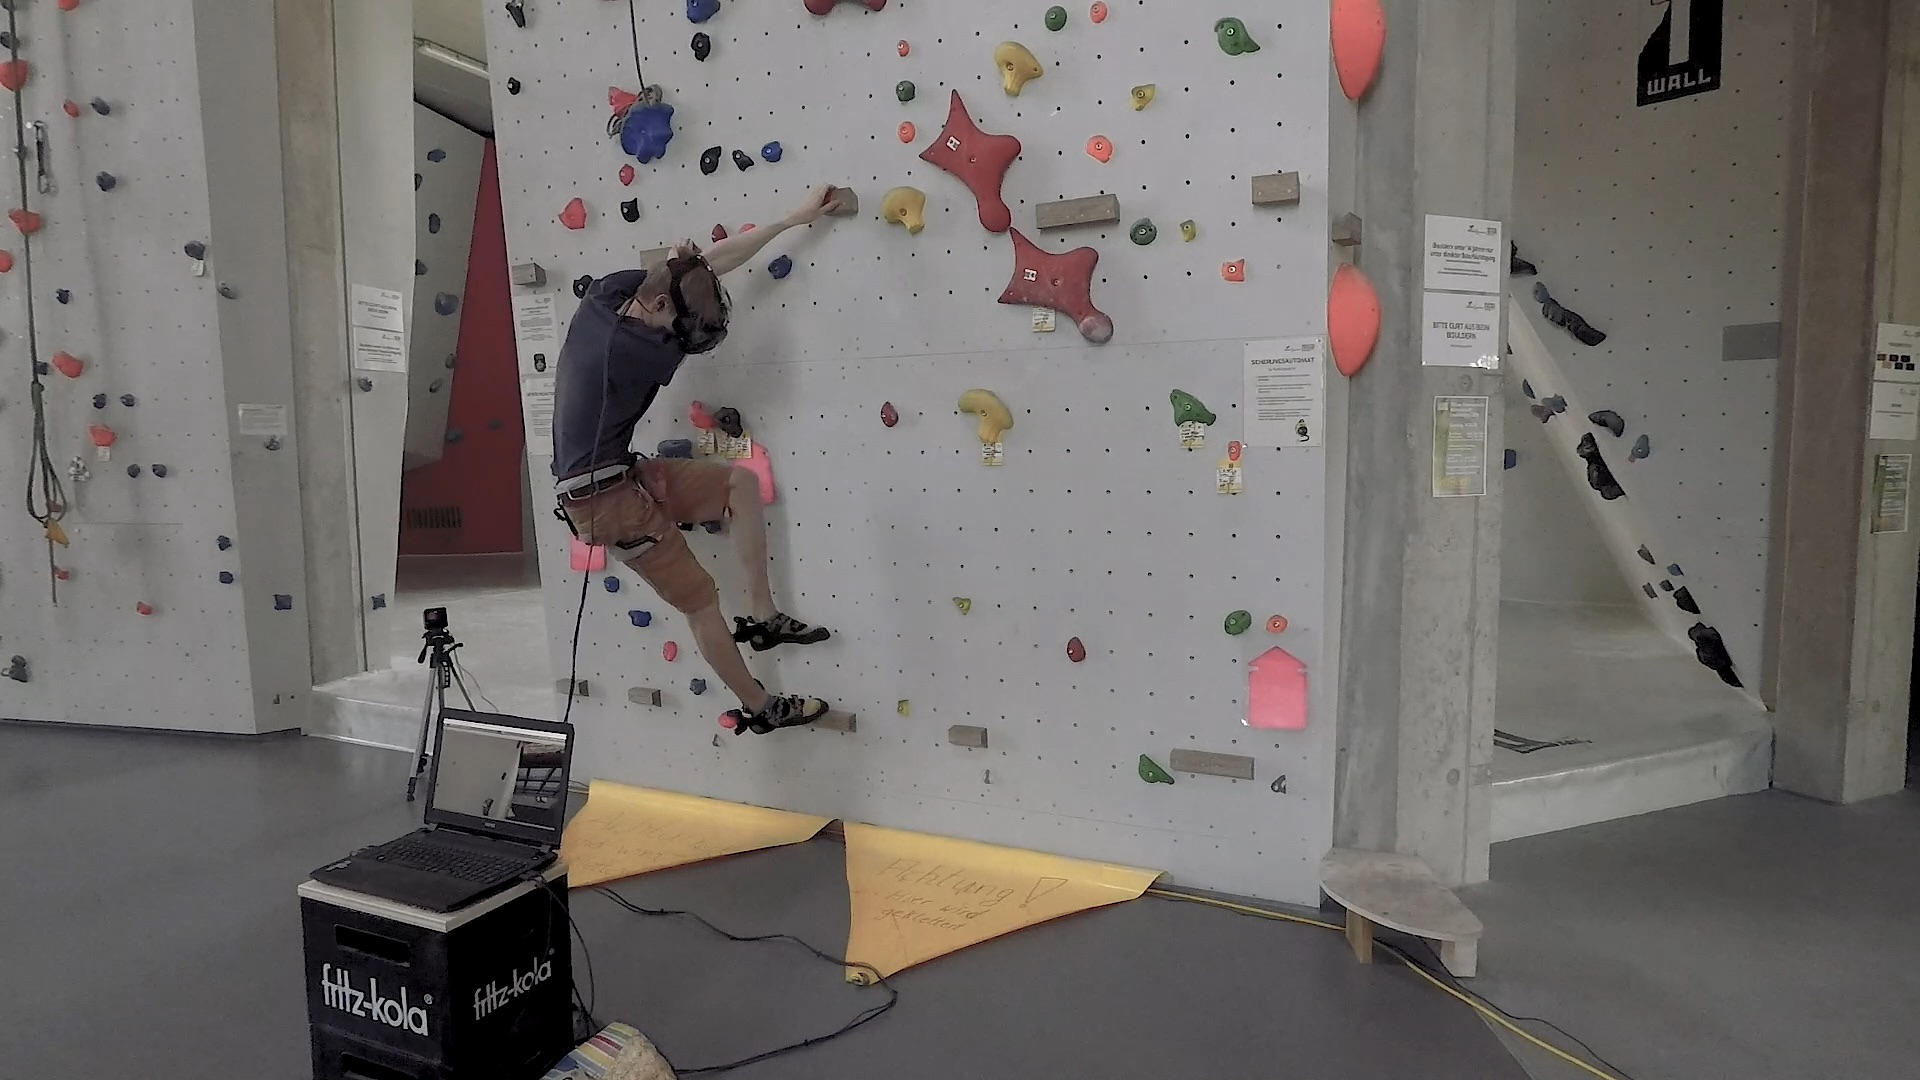
\includegraphics[width=\paperwidth]{include/images/master-thesis-clip-2.jpg}}{include/videos/master-thesis-clip-2.mov}}
	\begin{frame}[standout]
	\end{frame}
}

{
	\usebackgroundtemplate{\movie[label=clip-1,width=\paperwidth,height=\paperheight,open,once,showcontrols=false]{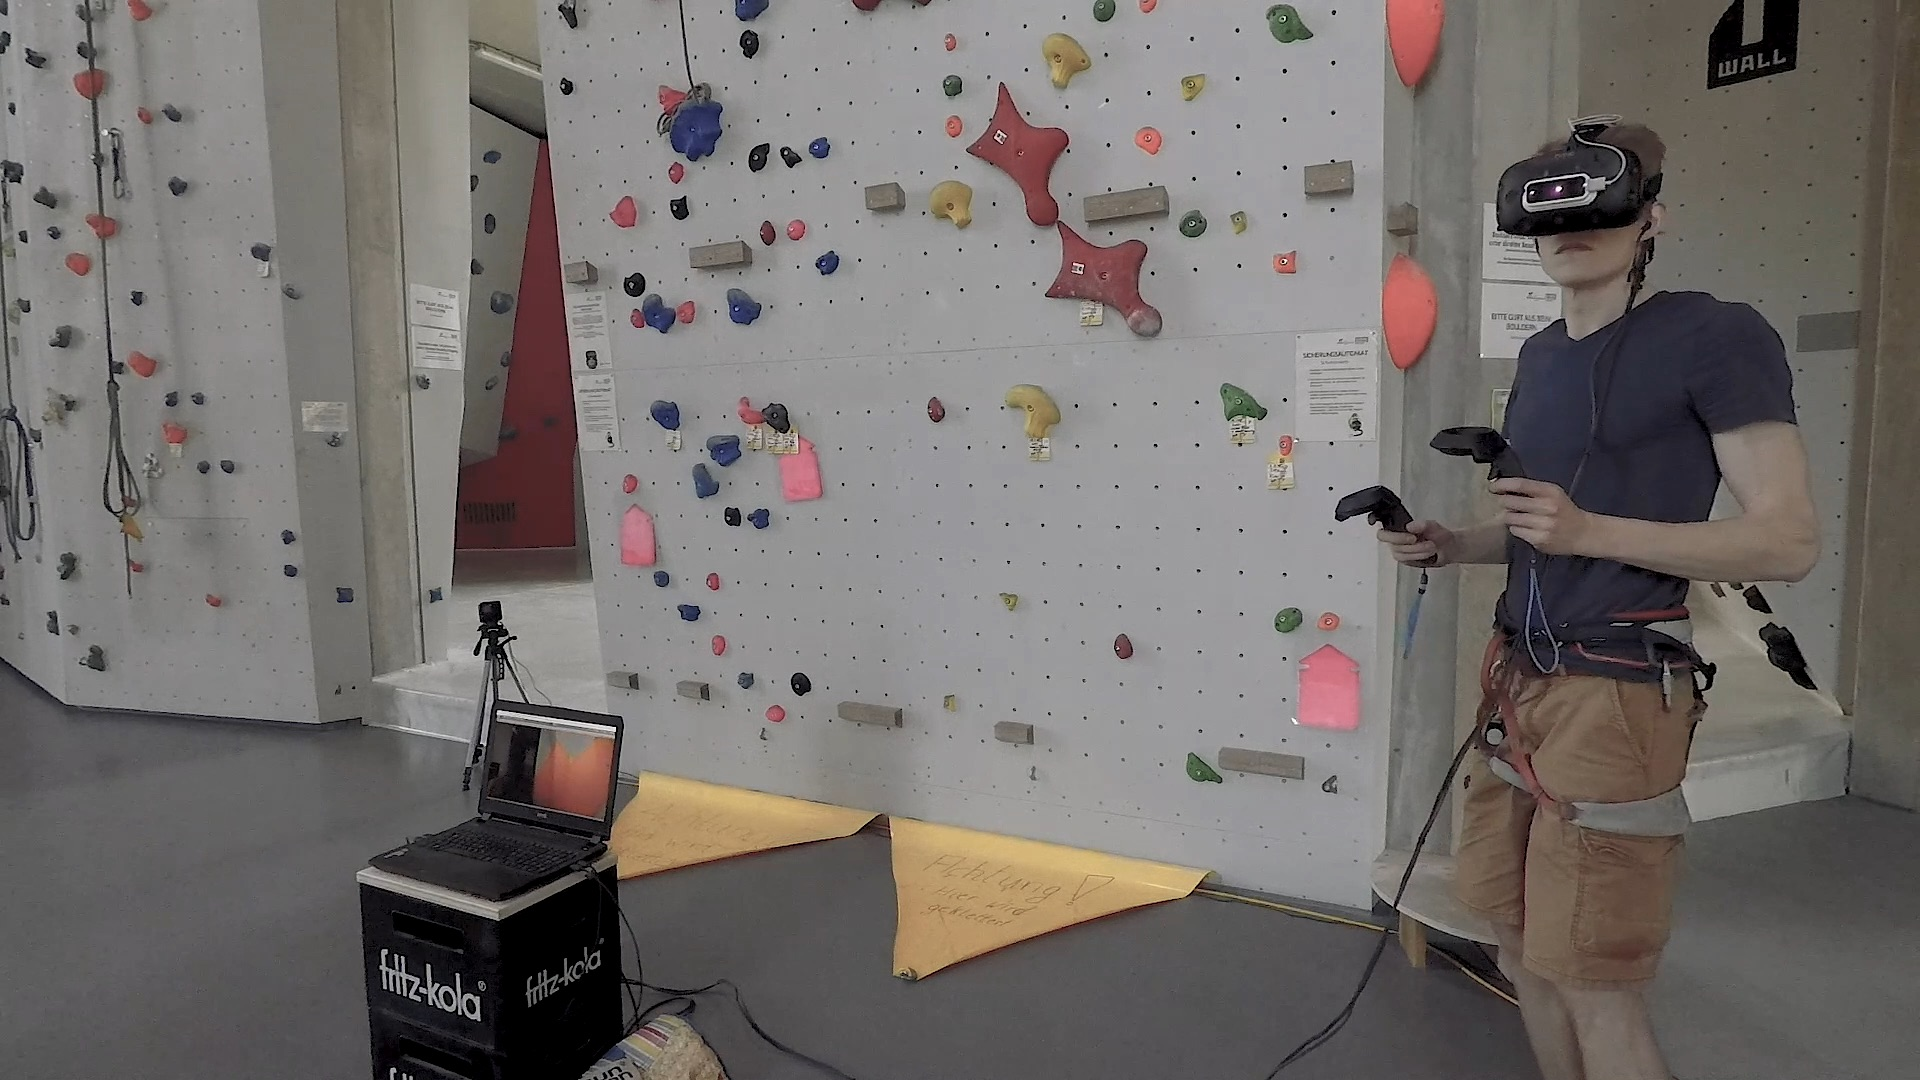
\includegraphics[width=\paperwidth]{include/images/master-thesis-clip-3.jpg}}{include/videos/master-thesis-clip-3.mov}}
	\begin{frame}[standout]
	\end{frame}
}

%\section{Studie}

\begin{frame}{Versuchsbedingungen}
\begin{columns}
	\begin{column}{0.5\textwidth}
		\begin{enumerate}[label=\textbf\textcolor{tertiary}{\Alph*}]
			\item Reales Klettern an Griffen und Tritten
			\\\textcolor{source}{\SI{10}{\meter} über Grund}
			\item Klettern in \gls{VR} an Griffen und Tritten
			\\\textcolor{source}{visuell \SI{10}{\meter} über Grund}
			\item Klettern in \gls{VR} mit Game Controllern
			\\\textcolor{source}{visuell \SI{10}{\meter} über Grund}
		\end{enumerate}
	\end{column}
	\begin{column}{0.5\textwidth}
		\begin{center}
			\vspace*{-15mm}
			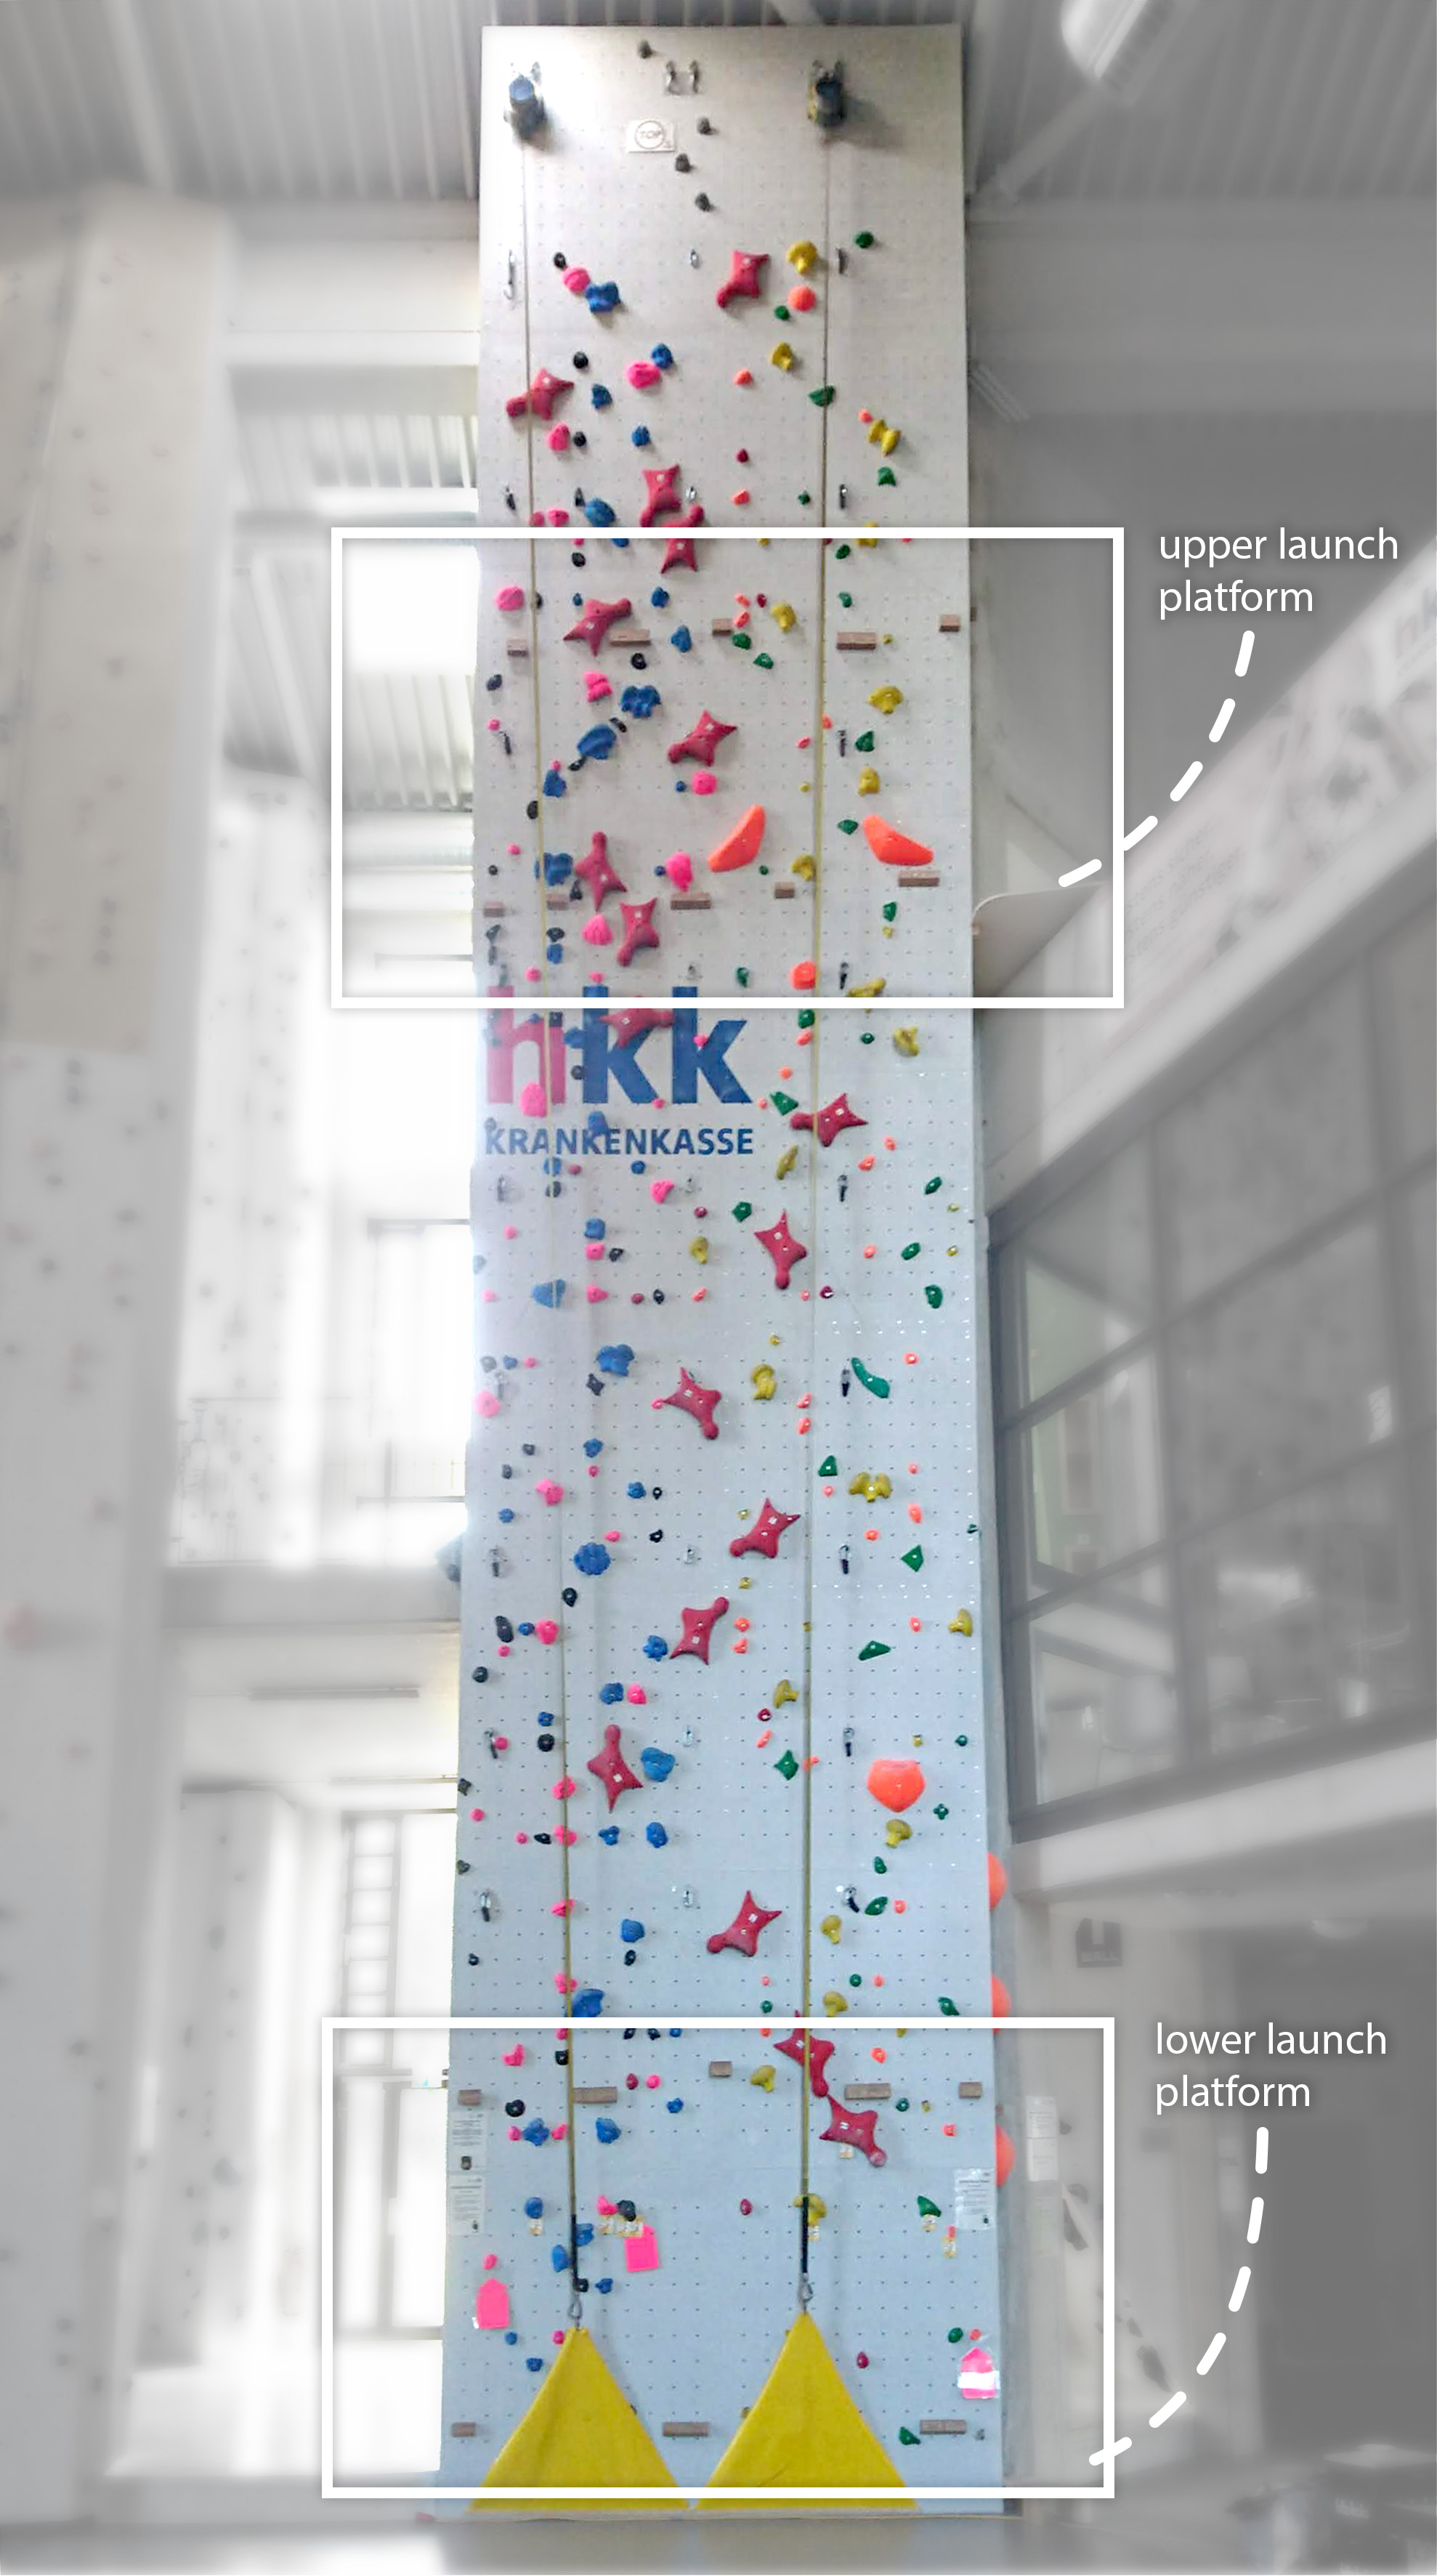
\includegraphics[height=1.2\textheight]{include/images/climbing-wall-photo.jpg}
		\end{center}
	\end{column}
\end{columns}
\end{frame}

\subsection{Technische Umsetzung}

\begin{frame}{\currentname{} -- Virtual Reality System}
	\begin{figure}
		\begin{subfigure}[t]{0.49\textwidth}
			\centering
			\begin{overpic}[width=\textwidth]{include/images/vive-kit.jpg}
				\rbox{-1}{1}{\textcolor{source}{\tiny{Quelle: \href{			https://www.inet.se/produkt/x107651/htc-vive}{HTC Corporation}}}}
			\end{overpic}
			\caption{HTC VIVE + Basistation + Controller}
		\end{subfigure}
		\begin{subfigure}[t]{0.49\textwidth}
			\centering
			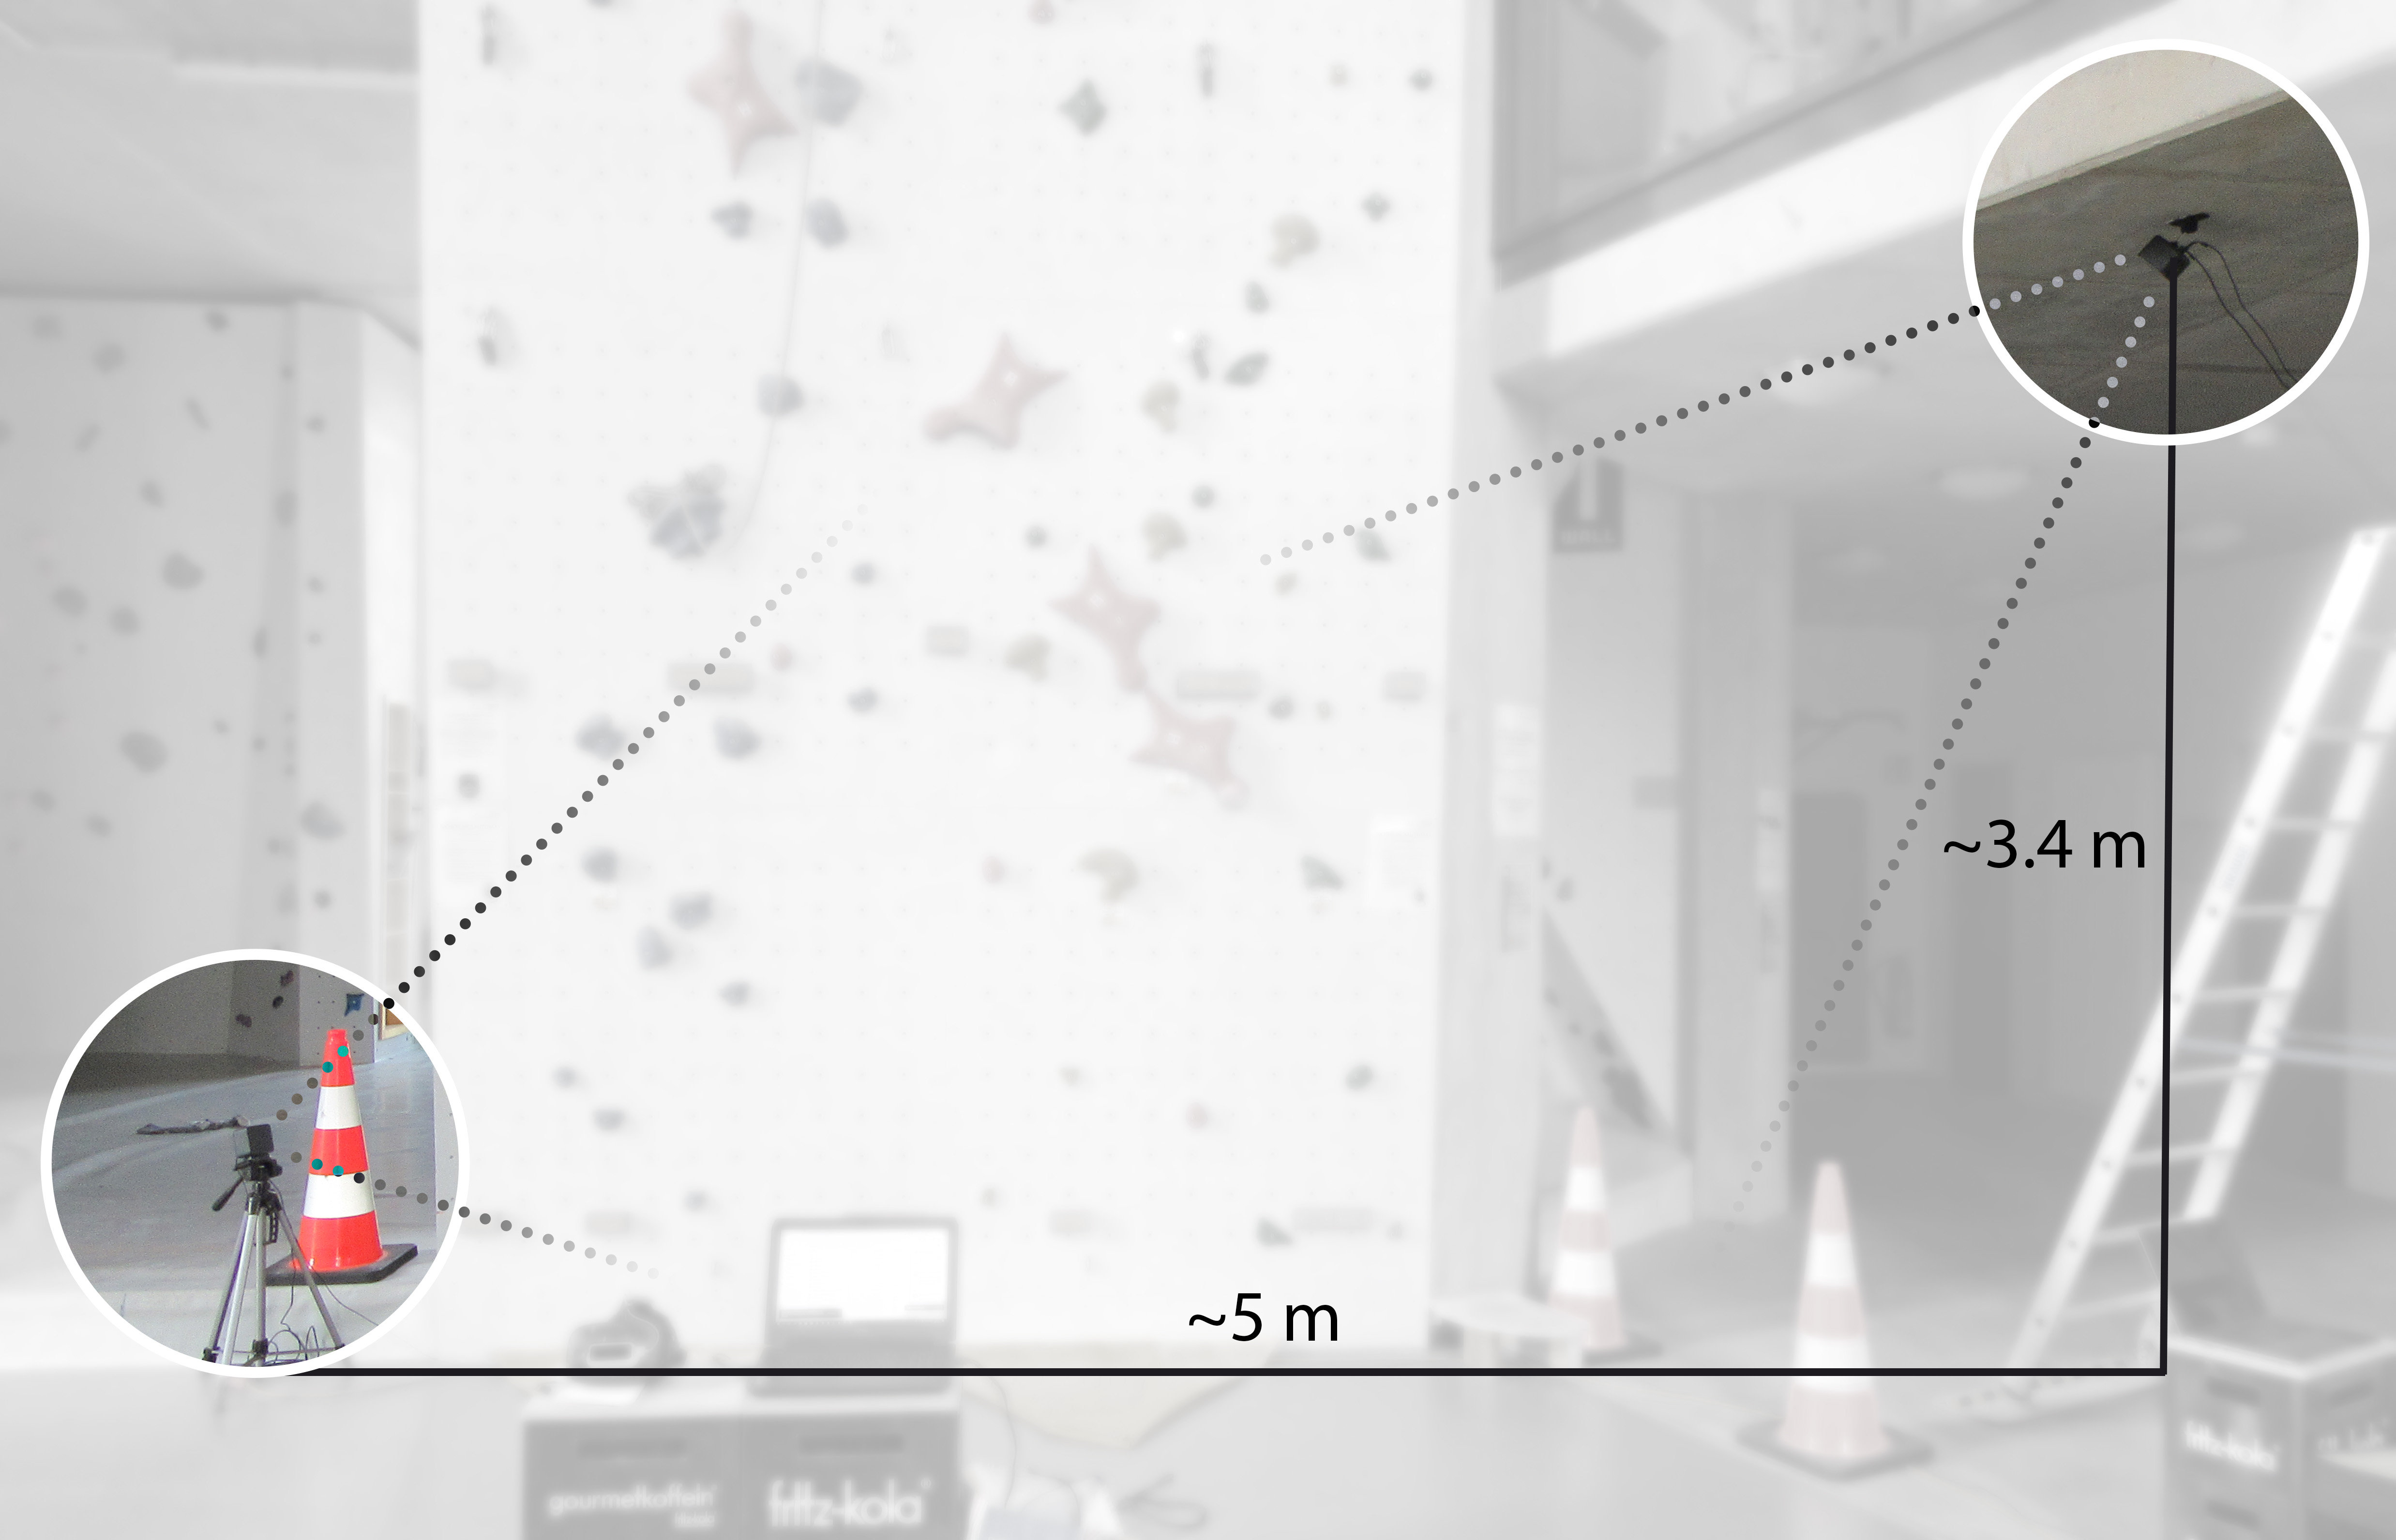
\includegraphics[width=\textwidth]{include/images/vive-setup-solution.jpg}
			\caption{HTC VIVE Position der Basistationen}
		\end{subfigure}
	\end{figure}
\end{frame}

\begin{frame}{\currentname{} -- Fuß Tracking}
\begin{figure}
	\centering
	\begin{subfigure}[t]{0.49\textwidth}
		\centering
		\includegraphics[width=\textwidth]{include/images/foot-tracking-tracker.png}
		\caption{VIVE Tracker befestigt an der Ferse}
		\label{fig:foot-tracking-tracker}
	\end{subfigure}
	\hfill
	\begin{subfigure}[t]{0.49\textwidth}  
		\centering 
		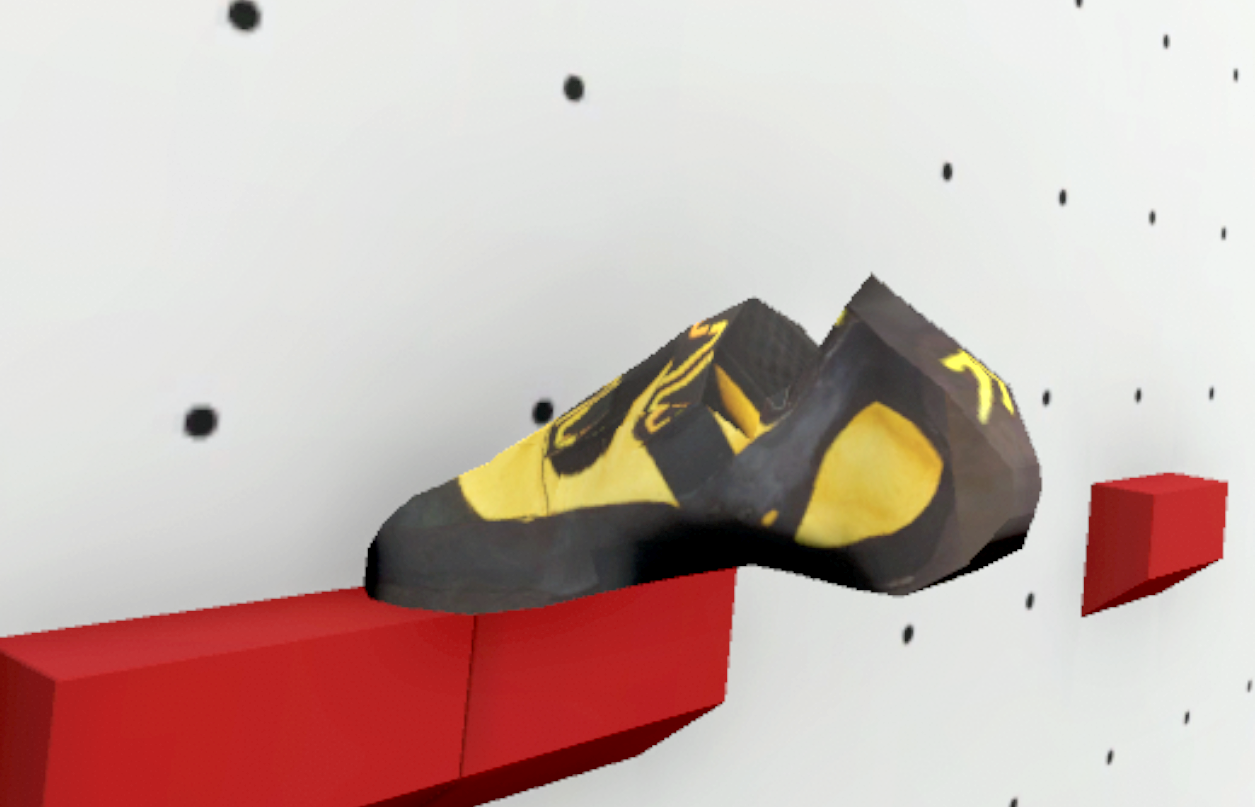
\includegraphics[width=\textwidth]{include/images/foot-tracking-result.png}
		\caption{Übertragenes Tracking auf 3D Modell in Unity}
		\label{fig:foot-tracking-result}
	\end{subfigure}
	\label{fig:foot-tracking}
\end{figure}
\end{frame}

\begin{frame}{\currentname{} -- Hand Tracking}
\begin{figure}
	\centering
	\begin{subfigure}[t]{0.32\textwidth}
		\centering
		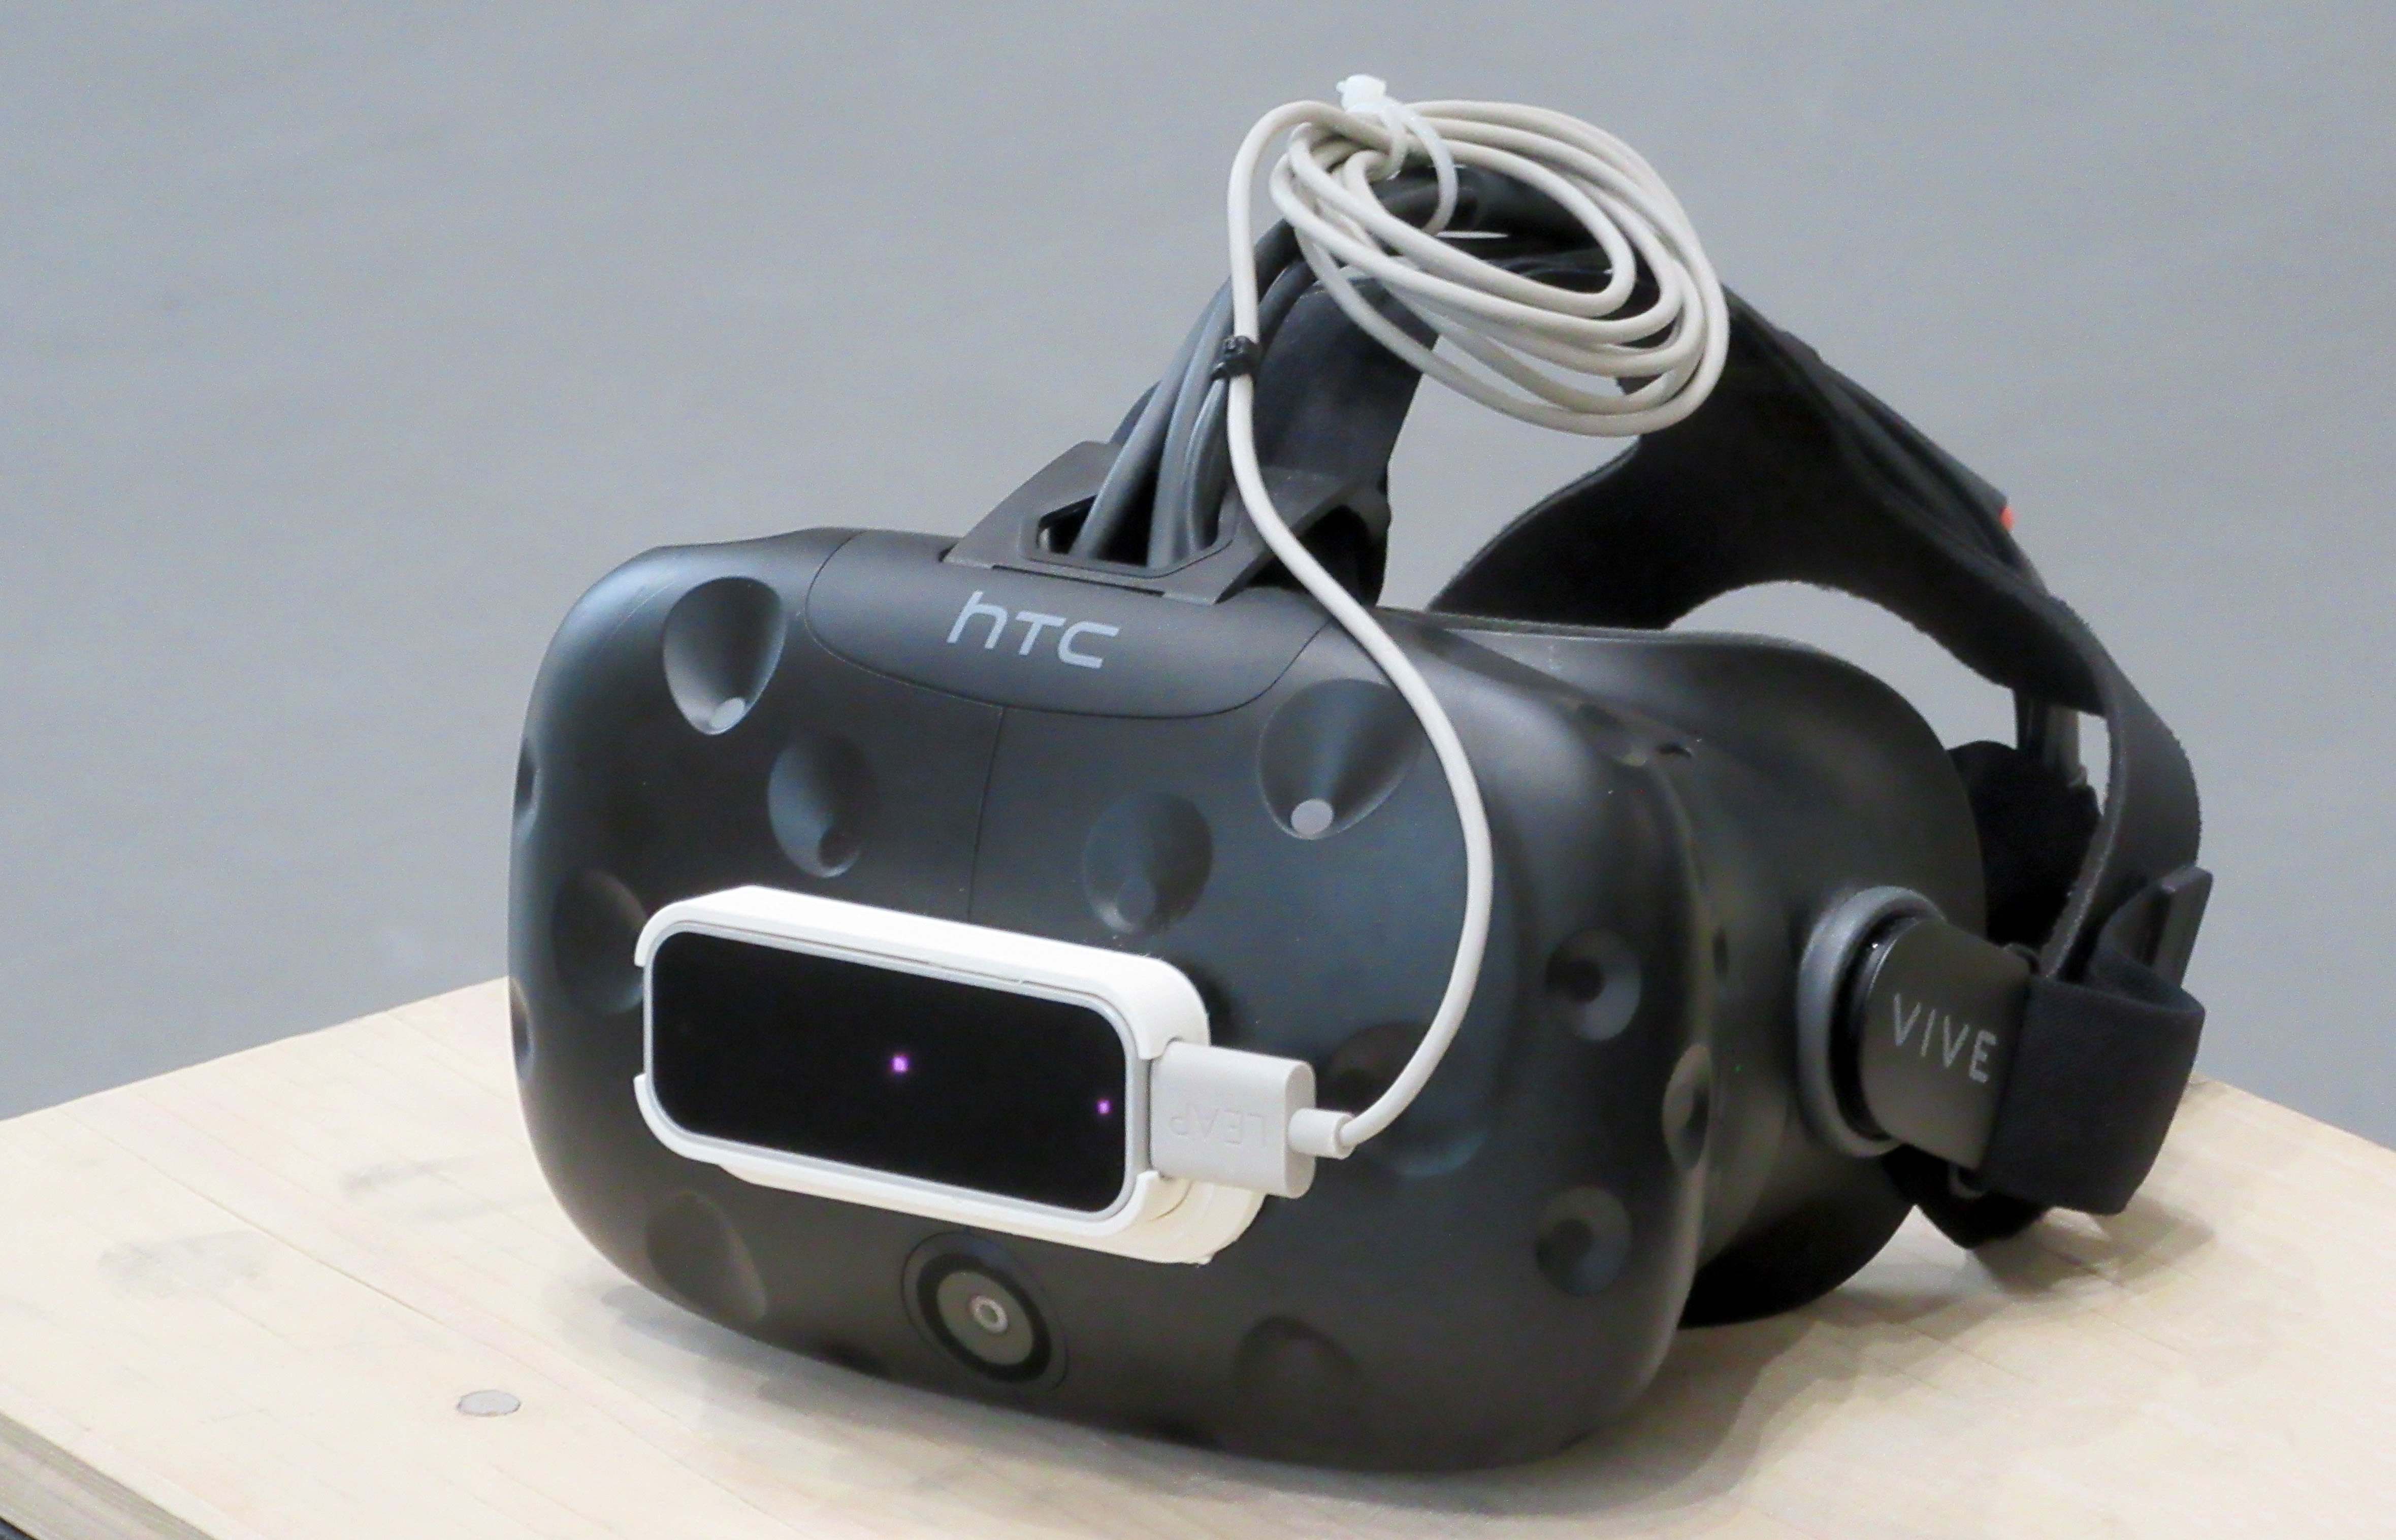
\includegraphics[width=\textwidth]{include/images/leap-motion-overlay-setup.jpg}
		\caption{LEAP Motion auf VIVE Headset}
		\label{fig:leap-motion-setup}
	\end{subfigure}
	\hfill
	\begin{subfigure}[t]{0.32\textwidth}
		\centering
		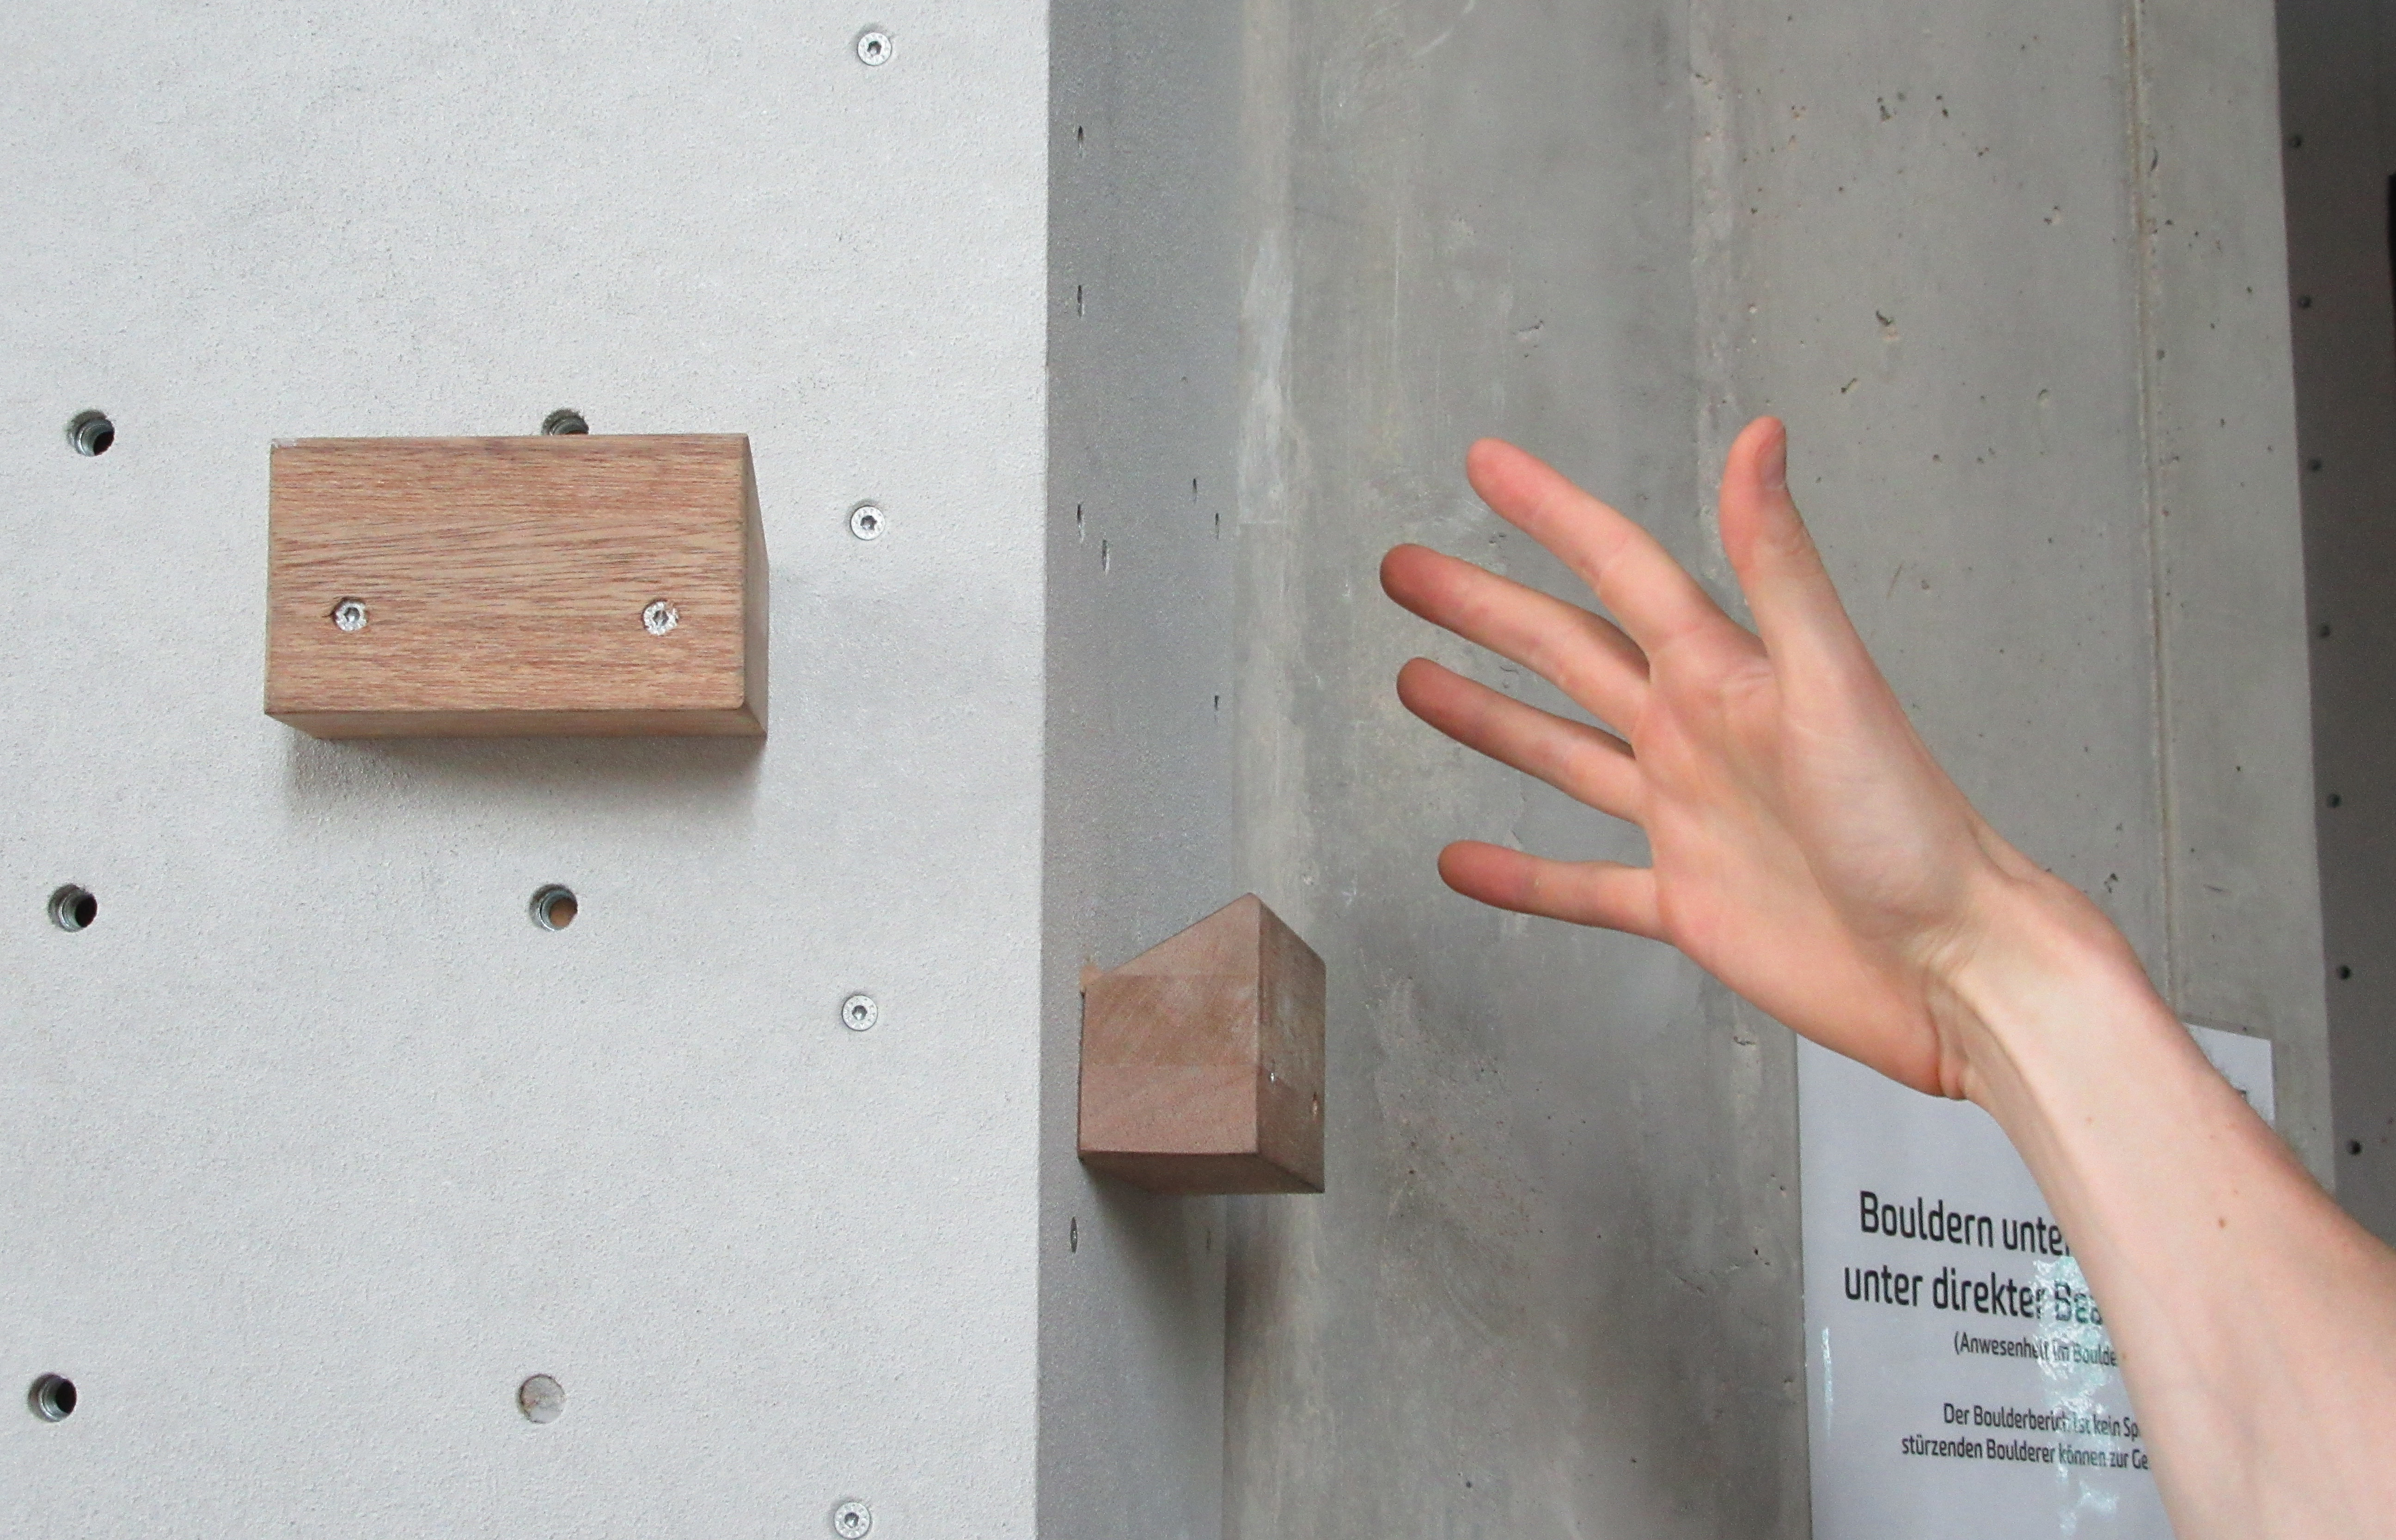
\includegraphics[width=\textwidth]{include/images/leap-motion-overlay-photo.jpg}
		\caption{Reale Perspektive (Foto)}
		\label{fig:leap-motion-overlay-photo}
	\end{subfigure}
	\hfill
	\begin{subfigure}[t]{0.32\textwidth}
		\centering
		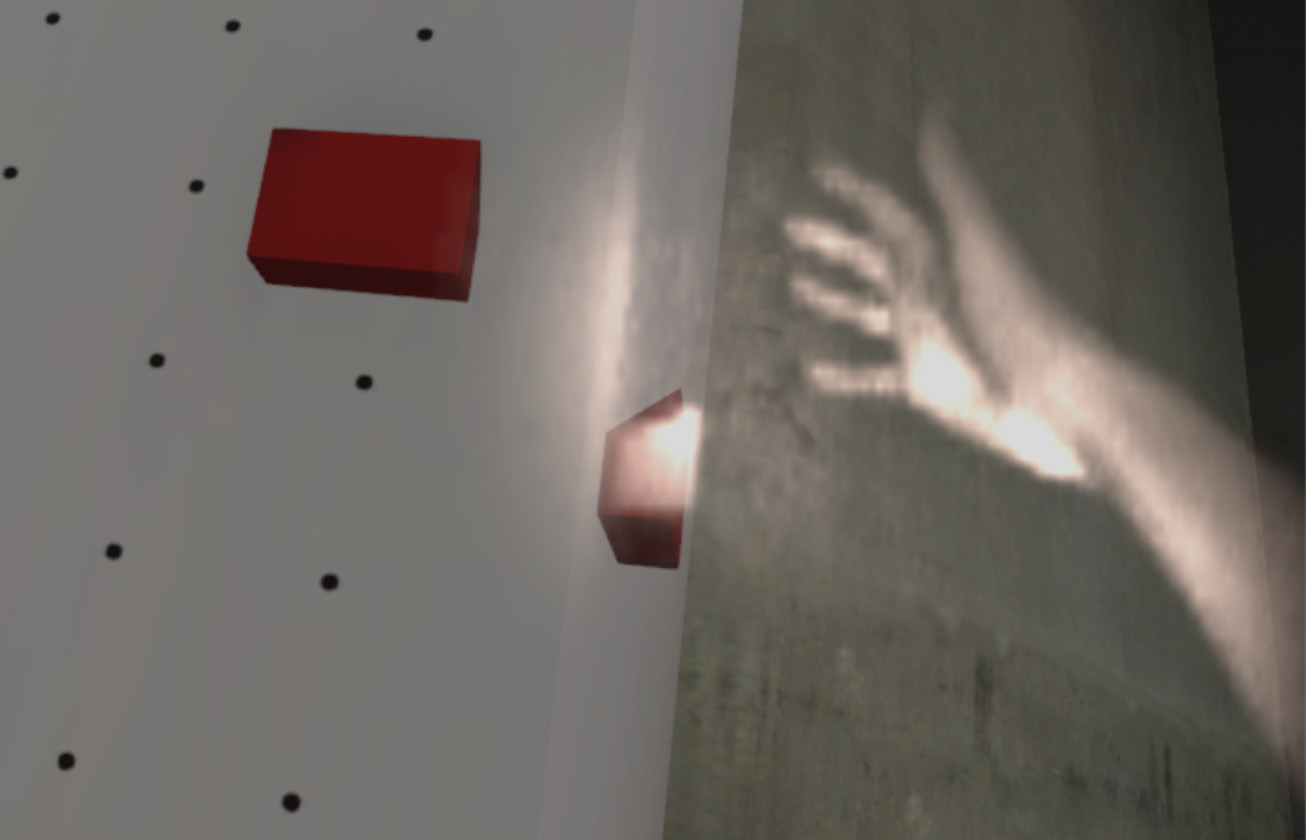
\includegraphics[width=\textwidth]{include/images/leap-motion-overlay-result.jpg}
		\caption{Resultierende des Overlays (Unity)}
		\label{fig:leap-motion-overlay-result}
	\end{subfigure}
	\captionsetup{subrefformat=parens}
	\caption[Leap Motion hand tracking]{Hand Overlay erzeugt aus einem Infrarotbild des LEAP Motion Sensors \subref{fig:leap-motion-setup} welches weich anhand des 3D Modells maskiert wird $\rightarrow$ nahegelegene Griffe bleiben sichtbar \subref{fig:leap-motion-overlay-result}}
	\label{fig:leap-motion-overlay}
\end{figure}
\end{frame}

\begin{frame}{\currentname{} -- Biosignalerfassung}
\begin{figure}
	\centering
	\begin{subfigure}[b]{0.49\textwidth}
		\centering
		{
			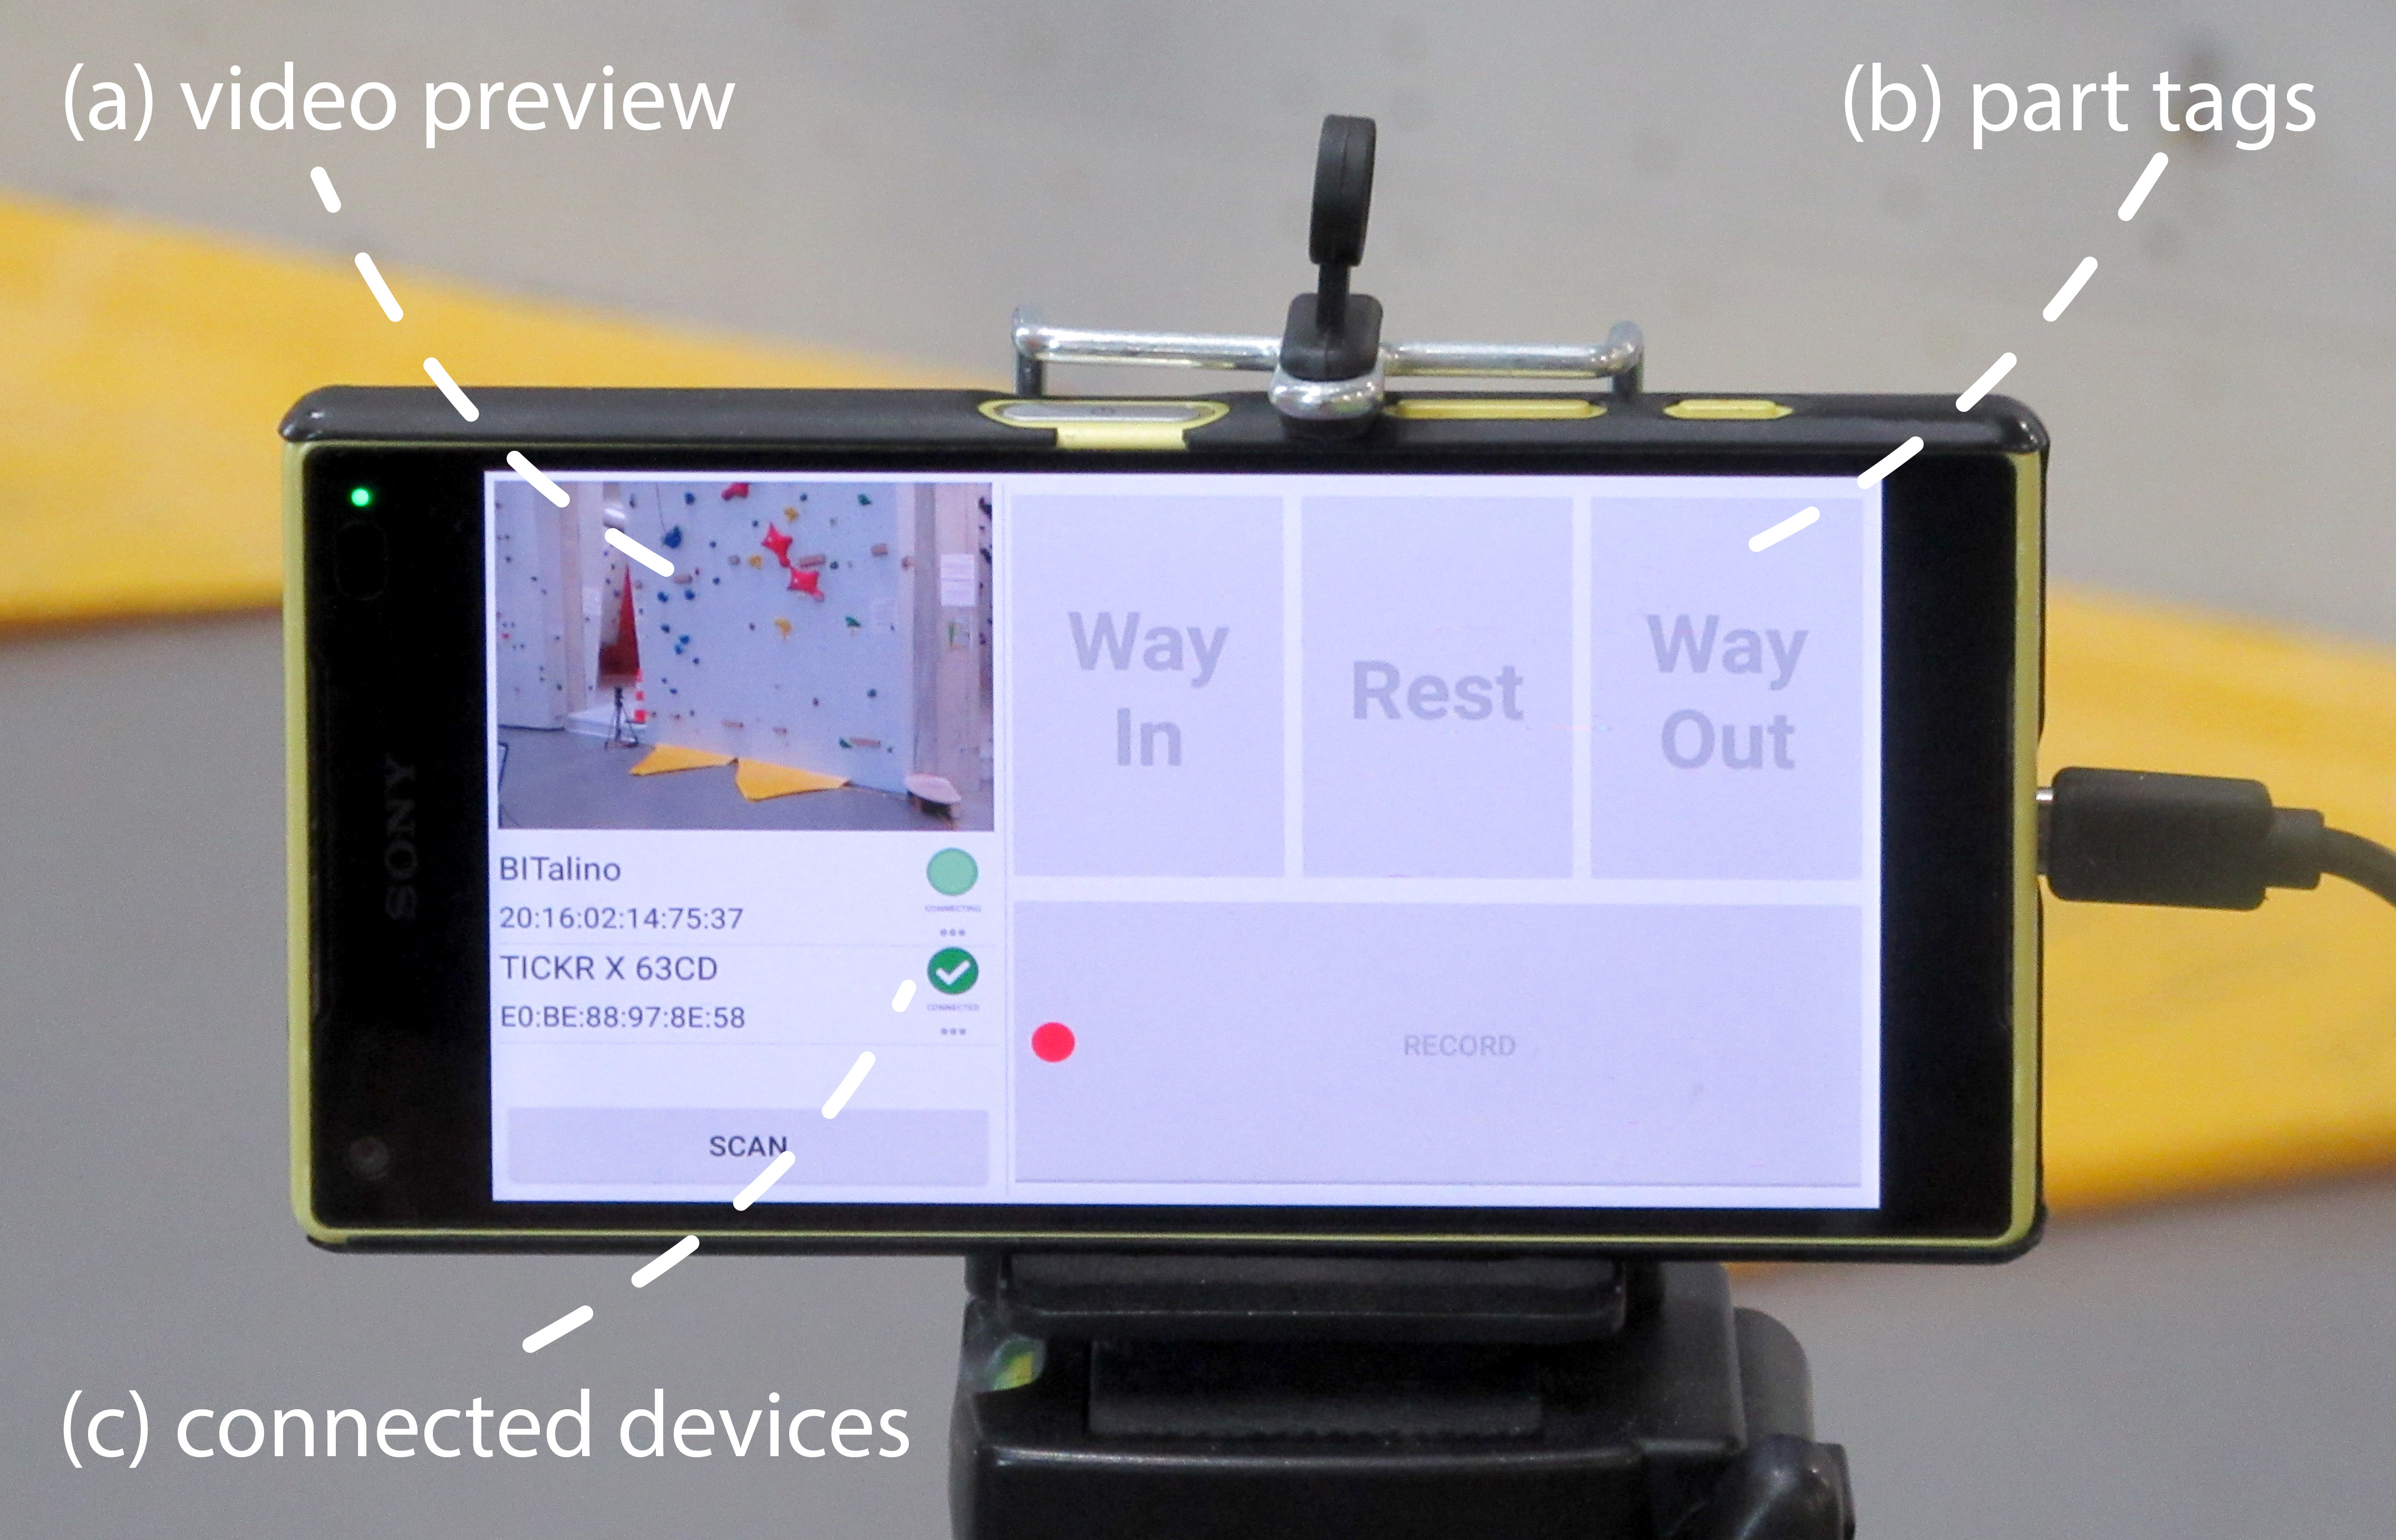
\includegraphics[width=\textwidth]{include/images/android-app-photo.jpg}
			\phantomsubcaption\label{fig:android-app-preview}
			\phantomsubcaption\label{fig:android-app-parts}
			\phantomsubcaption\label{fig:android-app-devices}
		}
		\captionsetup{subrefformat=parens}
		\caption{Android App zur Erfassung der Biosignale, mit Videovorschau \subref{fig:android-app-preview}, einer Liste verbundener Sensoren \subref{fig:android-app-devices} und Knöpfen zum Markieren der Versuchsabschnitte \subref{fig:android-app-parts}}
		\label{fig:android-app}
	\end{subfigure}
	\hfill
	\begin{subfigure}[b]{0.49\textwidth}  
		\centering
		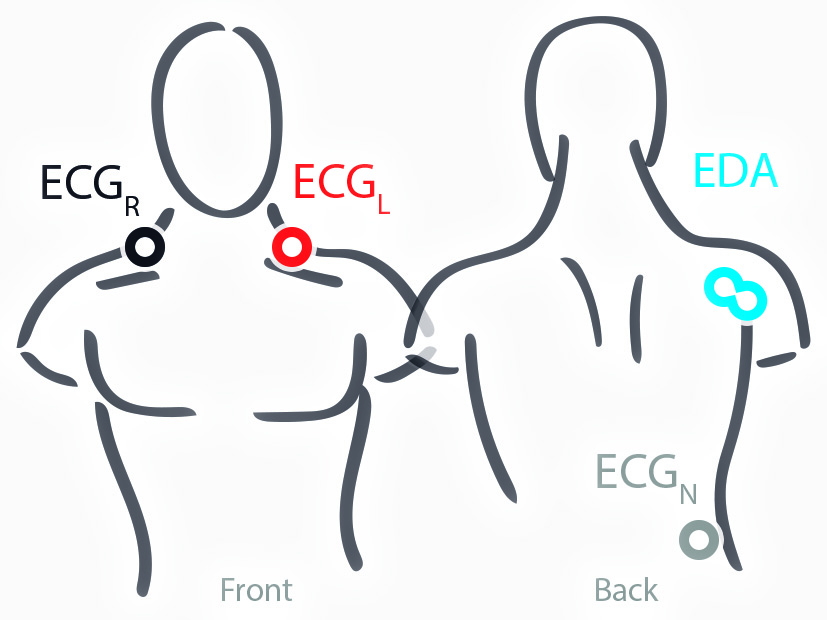
\includegraphics[width=\textwidth]{include/images/electrodes.jpg}
		\caption{Schematische Übersicht zur Platzierung Elektroden für ECG (Herzschlag) und EDA (Hautleitfähigkeit) in Anlehnung an \textcite{ECGLeadPlacement2015}}
		\label{fig:electrodes-schema}
	\end{subfigure}
	\label{fig:biosignals}
\end{figure}
\end{frame}

\subsection{Ergebnisse}

\begin{frame}{\currentname{} -- Teilnehmer*innen}
	\begin{itemize}[label=\textcolor{tertiary}{\faicon{caret-right}}]
		\item 28 (13 w, 15 m) Teilnehmer*innen, 
		\item Alter: 30,7 Jahre (SD = 10.6)
		\item Können: Vorstieg (23), 6+ (± 1 Grad); Top-Rope (5), 5+/6- (±1 Grad) \textcolor{source}{Skala: UIAA}
		\item VR Vorerfahrung: keine (13), minimal (13), selten (2)
		\item keine überdurchschnittliche Ängstlichkeit (nach STAI-T)
		\item keine klinische Höhenangst (nach vHI)
	\end{itemize}
\end{frame}

\begin{frame}{\currentname{} -- Vergleichbarkeit}
	\begin{tabbing}
		\textcolor{primary}{\faicon{question-circle}} \quad \= \large Welchen Effekt hat die Bedingung (Griffe/Tritte|Controller) auf Präsenz/Angst?
	\end{tabbing}
	\begin{figure}[htb]
	\centering
	\begin{subfigure}[t]{0.49\columnwidth}
		\centering
		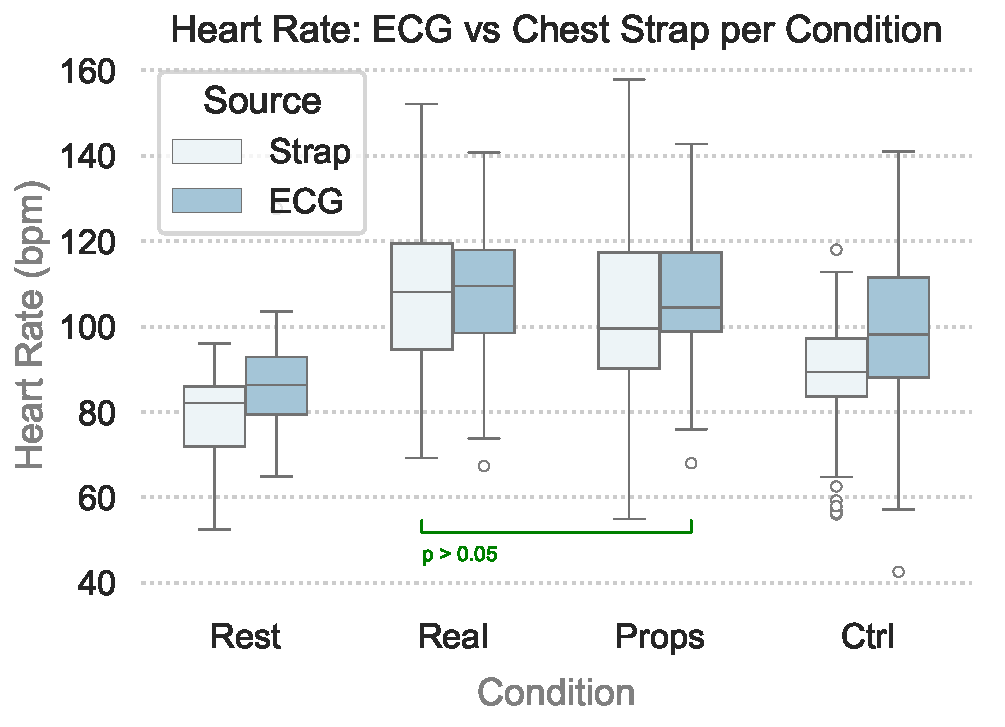
\includegraphics[width=\textwidth]{include/images/hr_per_condition_by_source.pdf}
		\label{fig:physical-exertion-hr}
	\end{subfigure}
	\hspace*{\fill}
	\begin{subfigure}[t]{0.49\columnwidth}
		\centering
		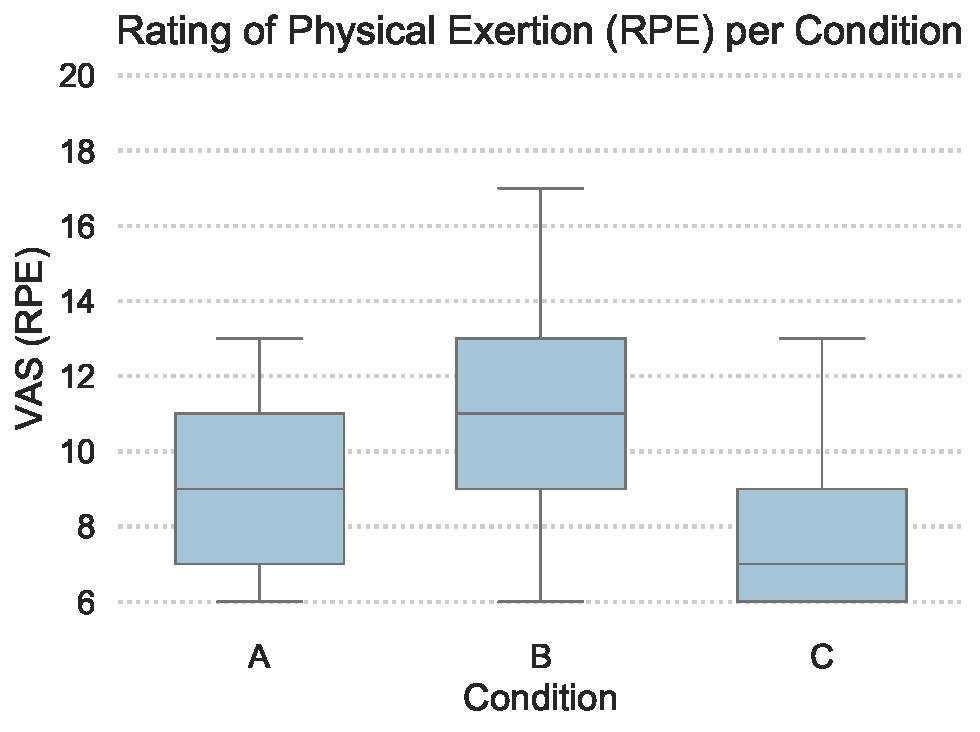
\includegraphics[width=\textwidth]{include/images/rpe_per_condition.pdf}
		\label{fig:physical-exertion-rpe}
	\end{subfigure}
	\label{fig:physical-exertion}
\end{figure}
\end{frame}

\begin{frame}{\currentname{} -- Angst}
\begin{figure}[htb]
	\centering
	\begin{subfigure}[t]{0.49\columnwidth}
		\centering
		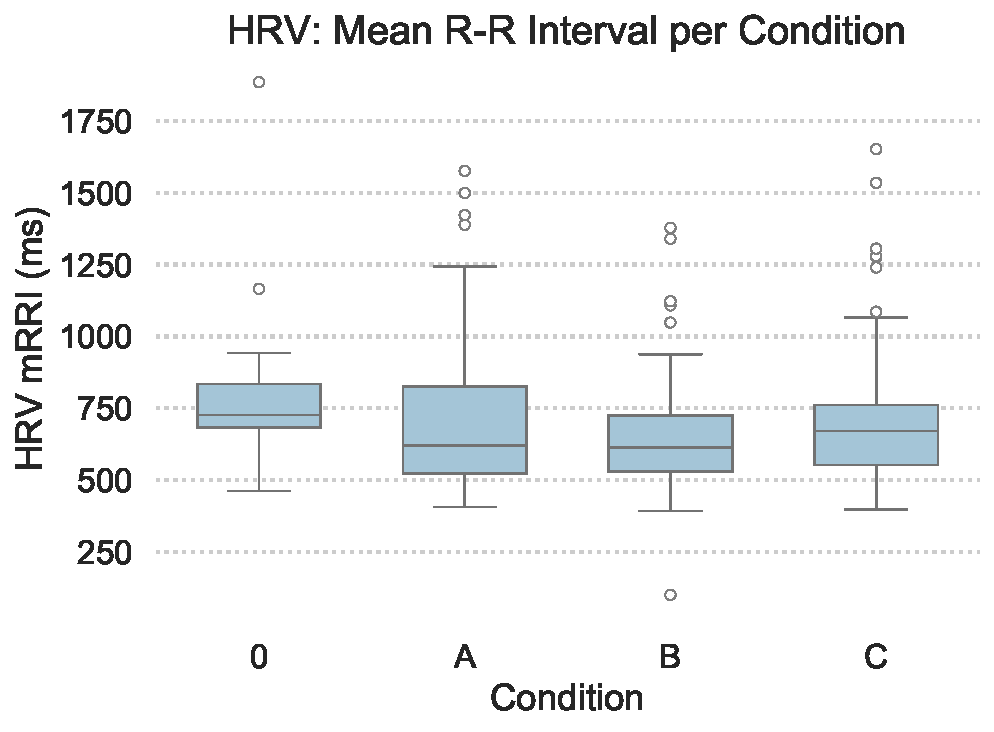
\includegraphics[width=\textwidth]{include/images/hrv_per_condition.pdf}
		\label{fig:stress-hrv}
	\end{subfigure}
	\hspace*{\fill}
	\begin{subfigure}[t]{0.49\columnwidth}
		\centering
		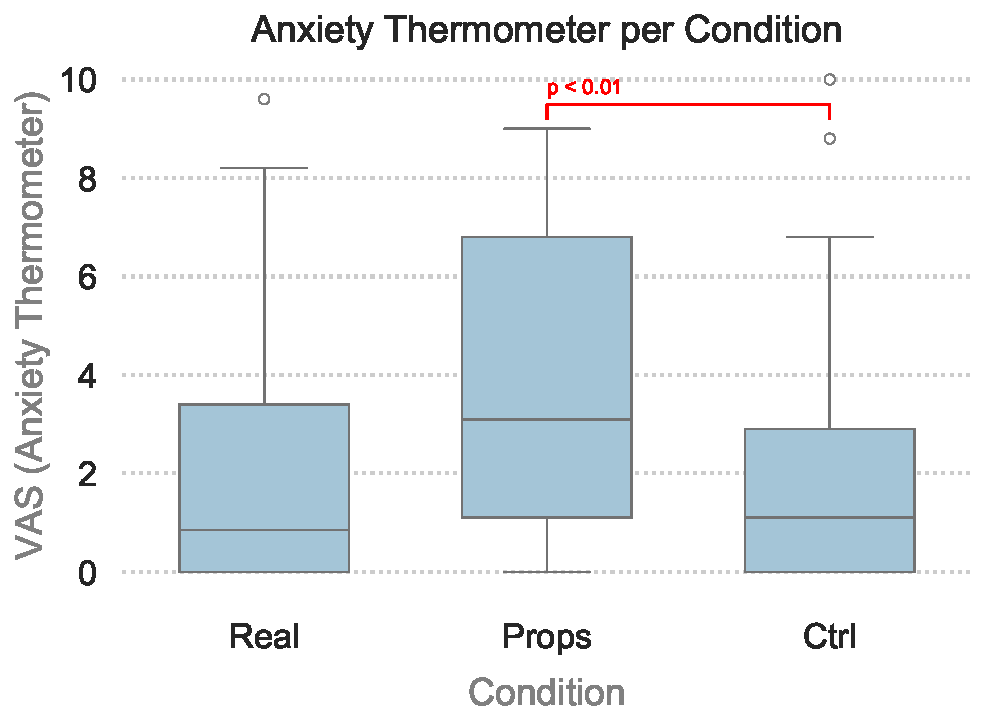
\includegraphics[width=\textwidth]{include/images/at_per_condition.pdf}
		\label{fig:anxiety-at}
	\end{subfigure}
	\label{fig:stress-anxiety}
\end{figure}
\end{frame}

\begin{frame}{\currentname{} -- Präsenz}
\begin{figure}[htb]
   \begin{center}
   	   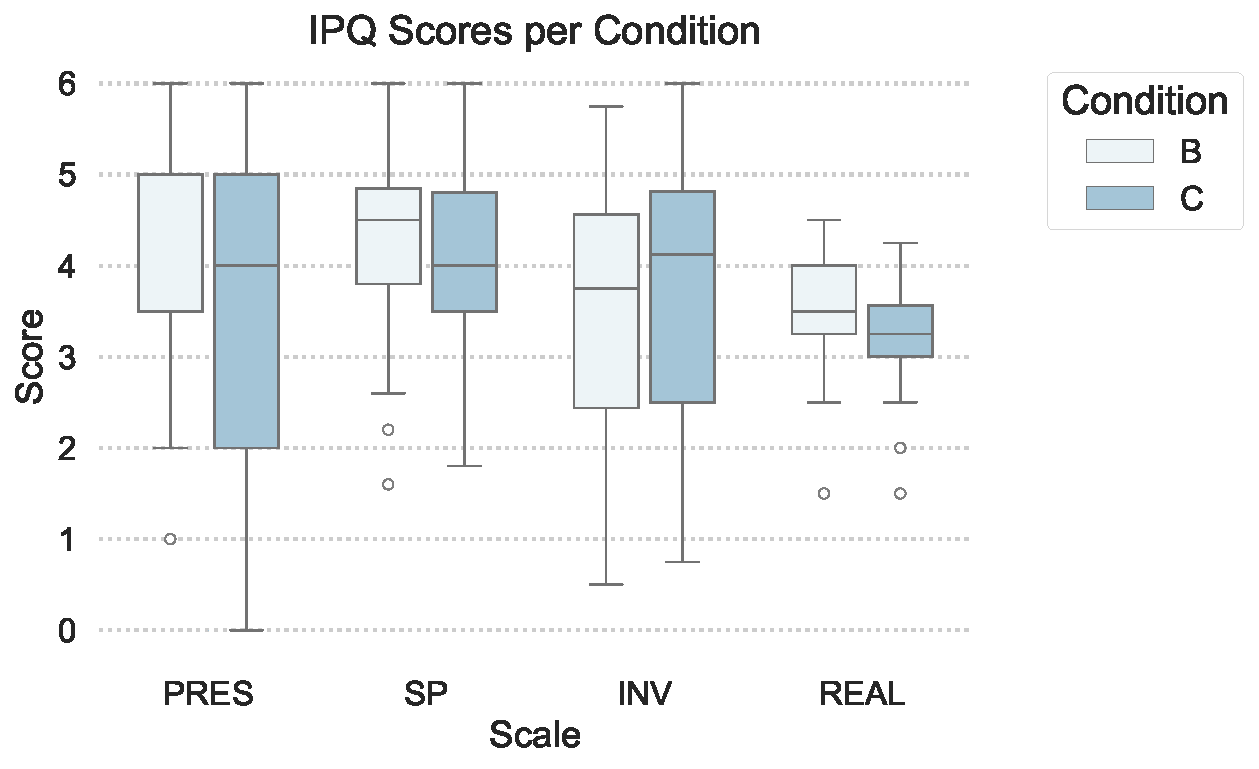
\includegraphics[width=0.6\textwidth]{include/images/ipq_per_condition}
   	\captionsetup{subrefformat=parens}
   	\caption{\gls{IPQ} Werte für die Bedingungen B und C auf den Skalen \textit{general presence} (PRES), \textit{spatial awareness} (SP), \textit{involvement} (INV), and \textcolor{secondary}{\textit{realness} (REAL)}}
   	\label{fig:presence}
   \end{center}
\end{figure}
\end{frame}

\subsection{Diskussion}

\begin{frame}{\currentname{} -- Mehrdeutigkeit}
\begin{tabbing}
	\textcolor{primary}{\faicon{question-circle}} \quad \= Welchen Effekt hat die Bedingung (Griffe/Tritte|Controller) auf Präsenz/Angst?
\end{tabbing}
\begin{description}
	\item[Präsenzerleben in VR \& Angst]\mbox{}
	\begin{itemize}
		\item[\textit{Psychologisch}] Griffe/Tritte $\rightarrow$ \textbf{erhöhte} Präsenz u. Angst\\
		\temporal<2>{\textcolor{white}{...}}{\textcolor{secondary}{Auslöser unklar, nicht zwingend Sturzangst}}{\textcolor{gray}{Auslöser unklar, nicht zwingend Sturzangst}}
		\item[\textit{Physiologisch}] \textbf{kein Unterschied} messbar zw. Griffe/Tritte|Controller\\
		\temporal<3>{\textcolor{white}{...}}{\textcolor{secondary}{Keine Änderung der Hautleitfähigkeit; Bewegungsartefakte?}}{Keine Änderung der Hautleitfähigkeit; Bewegungsartefakte?}
	\end{itemize}
\end{description}
\end{frame}

\subsection{Fazit und Ausblick}

{
	\setbeamertemplate{blocks}[default]
	\setbeamercolor{block title}{bg=secondary}
	\setbeamercolor{block body}{bg=white}
	\setbeamercolor{frametitle}{fg=primary,bg=}
	\addtobeamertemplate{block begin}{\pgfsetfillopacity{0.5}}{}
	\usebackgroundtemplate{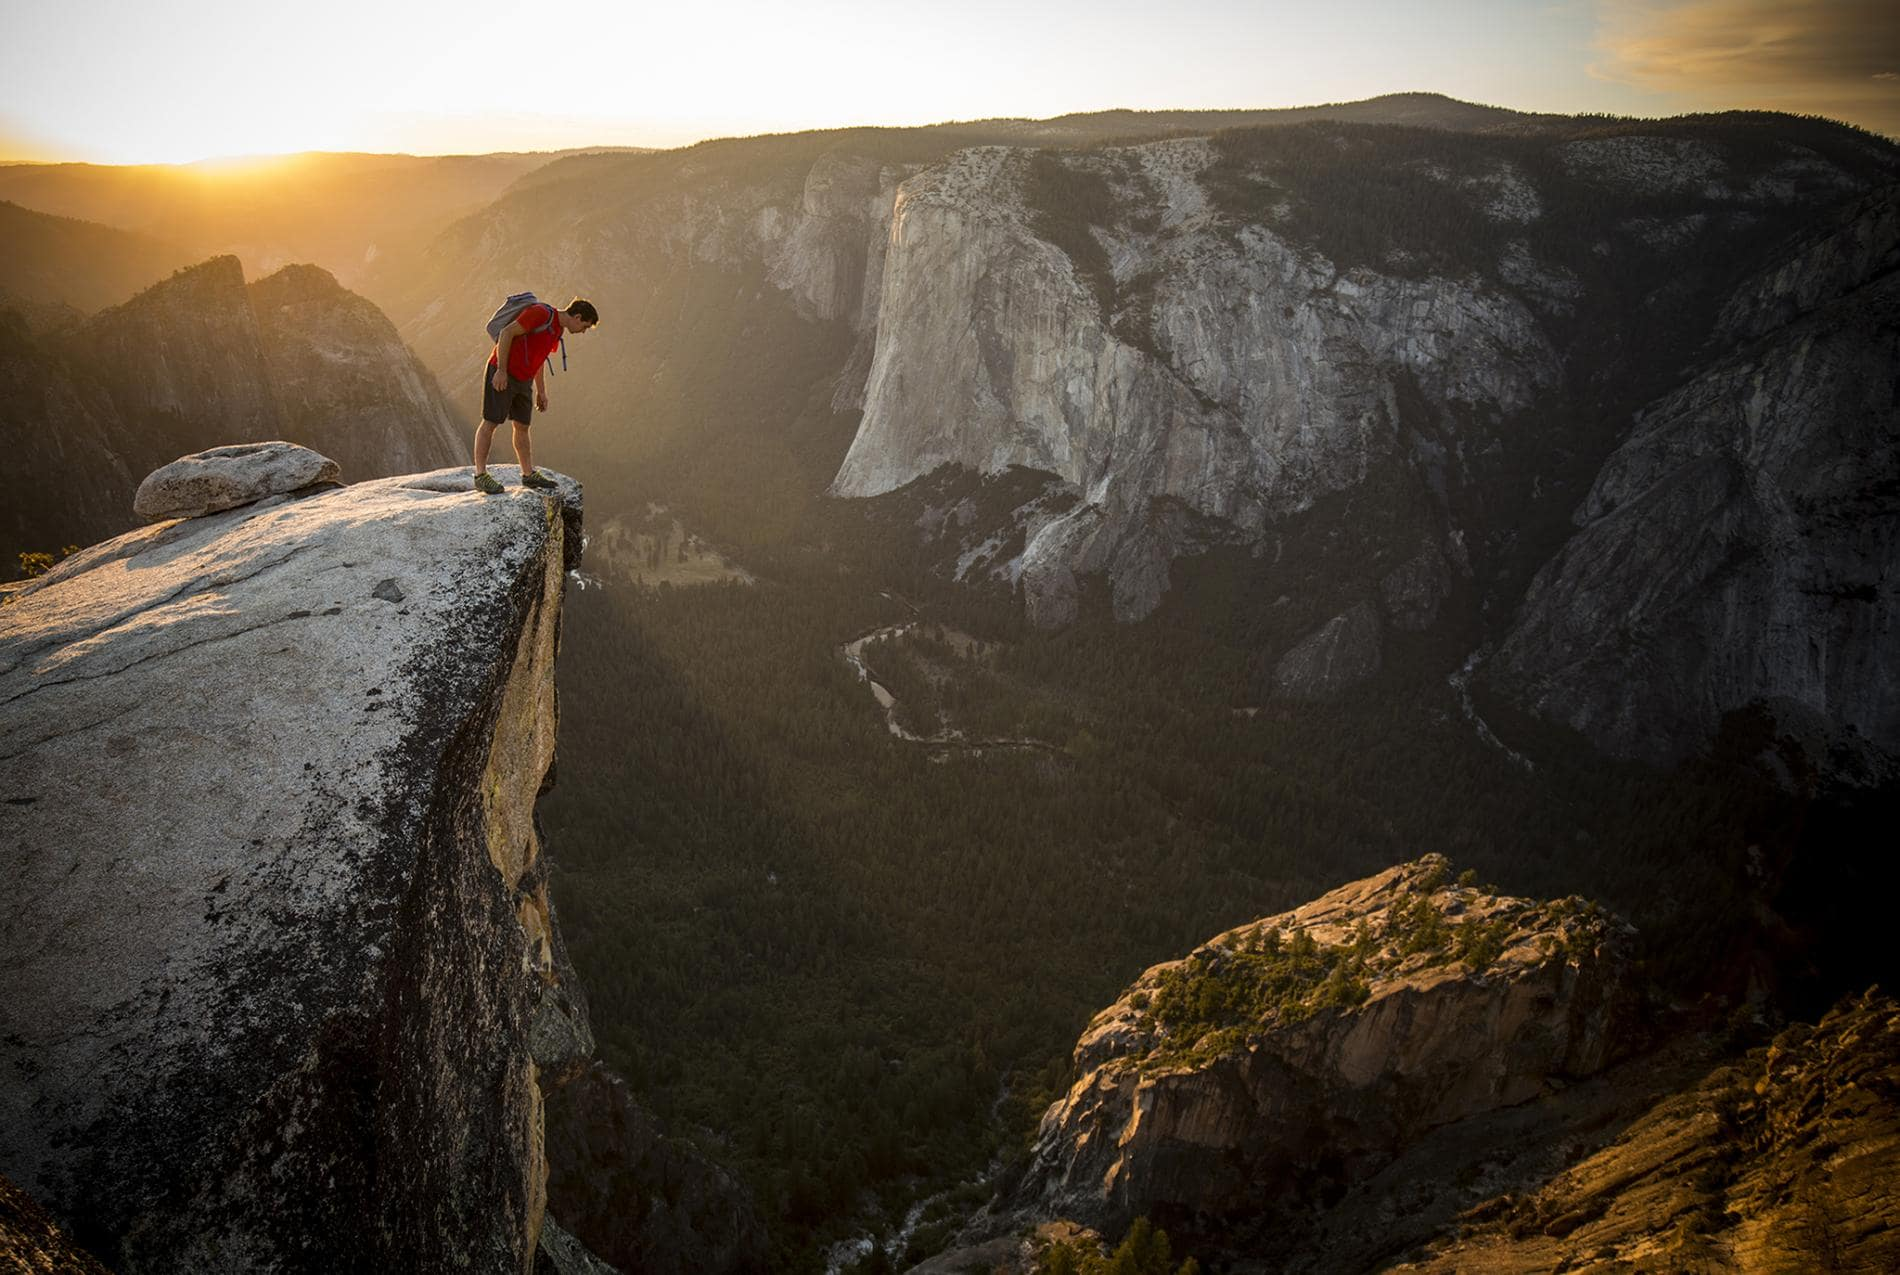
\includegraphics[width=\paperwidth]{include/images/alex-honnold-taft-point-yosemite-california.jpg}}
	\begin{frame}[plain]{\color{primary}{Fazit \& Ausblick}}
	
	\begin{columns}
		\begin{column}{0.4\textwidth}

		\end{column}
		\begin{column}{0.6\textwidth}
			\begin{exampleblock}{}<2->
				\textbf{Höhen-, Flug-, \textcolor{secondary}{und Sturzangst?}}
				\begin{itemize}[label=\textcolor{tertiary}{\faicon{caret-right}}]
					\item Ja und nein $\rightarrow$ mehr Forschung nötig\\zu Angst + physische Aktivität
				\end{itemize}
				\textbf{Technologischer Mehrwert}
				\begin{itemize}[label=\textcolor{tertiary}{\faicon{caret-right}}]
					\item neuartige, präzise Darstellung von Händen in VR\\zur physischen Interaktion
				\end{itemize}
				\textbf{Veröffentlichung auf der \textcolor{secondary}{CHI 2019}}
				\begin{itemize}[label=\textcolor{tertiary}{\faicon{caret-right}}]
					\item Weitere Arbeiten zu Klettern + VR
				\end{itemize}
			\end{exampleblock}
		\end{column}
	\end{columns}
	
	\begin{textblock}{50}(5,83)
		\href{http://www.accidentofgeography.com/alex-honnold-epic-el-capitan-triumph/}{	\textcolor{tertiary}{{\small \textcopyright Jimmy Chin}}} 
	\end{textblock}
	\end{frame}
}

\begin{frame}[plain]
\begin{center}
	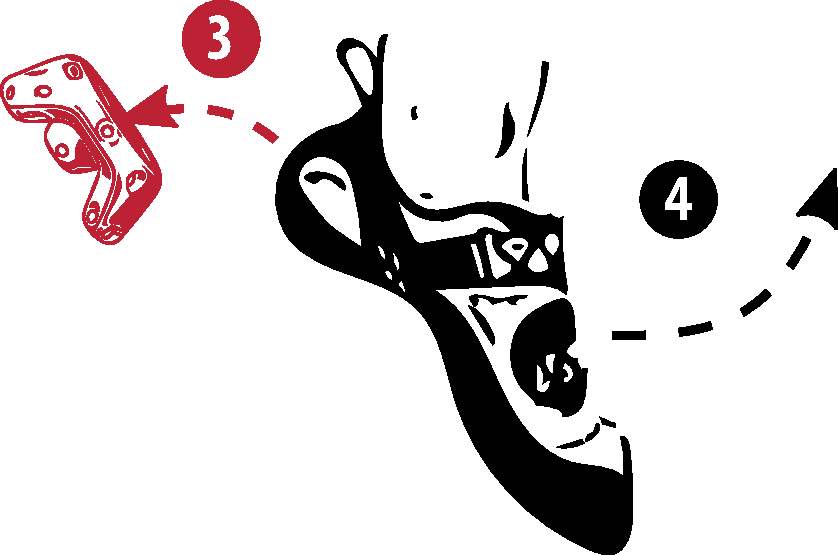
\includegraphics[width=0.8\textwidth]{include/images/climbing-shoe-with-instructions-off.pdf}
	\begin{textblock}{60}(20,58)
			
\includegraphics[width=\textwidth]{include/images/Logo-Grau.pdf}
	\end{textblock}
\end{center}
\end{frame}
